\chapter{Systematic Uncertainties}

Systematic uncertainty control is very important to and a highlight of these 2
high-precision experiments. To achieve a smaller systematic uncertainty, a
combination of fast-control and slow control was employed, which helped 
to cancel many systematic uncertainties brought by the accelerator to the
beam. Except the uncertainty from the machine, another important source
of systematic uncertainties is the detection process, namely the 
acceptance function.

After removing false asymmetry from the beam, we need further correction of the
background asymmetry, namely, target contamination and inelastic scattering,
as shown in Eq.~\ref{eq:background_correction}.
\begin{equation}
    \CA_{pv} = \frac{\CA_{cor}/\CP - \sum_i \CA_i f_i}{1 - \sum_i f_i}
    \label{eq:background_correction}
\end{equation}
Here, $\CA_i$ and $f_i$ refer to the asymmetry and rate fraction of background
processes. In PREX-II, contamination from the diamond foil contributed the
largest background correction.

The uncertainty propagation
\begin{equation}
    (\delta \CA_{pv})^2 = 
      \left( \frac{\partial \CA_{pv}}{\partial \CA_{cor}} \delta \CA_{cor} \right)^2
      + \left( \frac{\partial \CA_{pv}}{\partial \CP} \delta \CP \right)^2
      + \sum_i \left[ \left(\frac{\partial \CA_{pv}}{\partial \CA_i}\delta \CA_i \right)^2 
	 + \left(\frac{\partial \CA_{pv}}{\partial f_i}\delta f_i \right)^2 \right]
\end{equation}

\begin{equation}
    \frac{\partial \CA_{pv}}{\partial \CA_j} = -\frac{f_j}{1 - \sum_i f_i}  \qquad
    \frac{\partial \CA_{pv}}{\partial f_j} = \frac{\CA_{pv} - \CA_j}{1 - \sum_i f_i}
    \label{eq:systematic_uncertainty}
\end{equation}

%%%%%%%%%%%%%%%%%%%%%%%%%%%%%%%%%%%%%%%%%%%%%%%%%%%%%%%%%%%%%%%%%%%%%%%%
\section{$Q^2$ and $\theta$}
Physical interpretation of $\CA_{PV}$ requires precise knowledge
of the scattering angle and corresponding $Q^2$, which were determined using
a watercell target. 
\begin{figure}
    \centering
    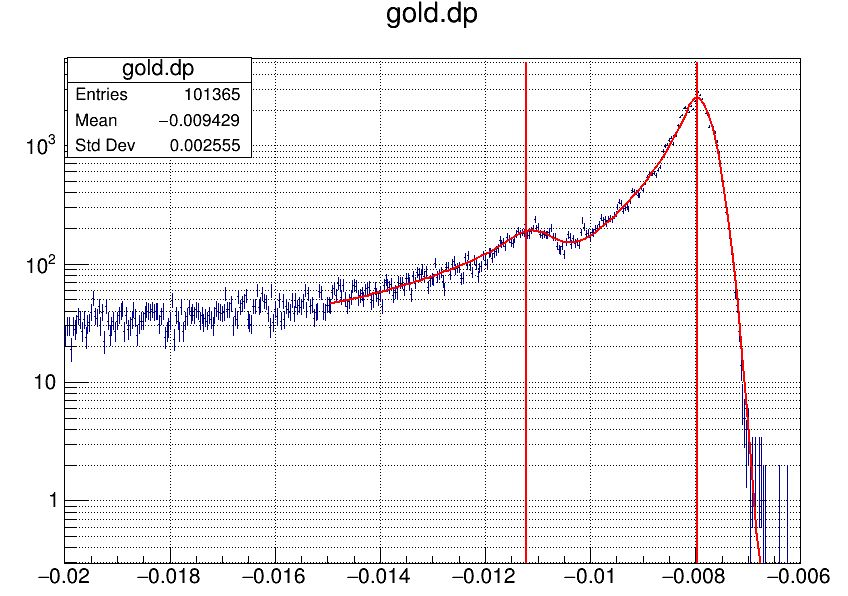
\includegraphics[width=0.5\linewidth]{watercell_Dp}
    \caption{Momentum distribution of the optics run with watercell. The x-axis
    is the relative energy difference: $dp = \frac{p - p0}{p0}$. Plot from Siyu}
    % HRS_optics_siyu
\end{figure}
As we see from Eq.~\ref{eq:scattered_energy}, the energy difference between the
2 elastic peaks is
\begin{equation}
    \Delta E' = E'_O - E'_H = E\left( \frac{1}{1 + \frac{E(1-\cos\theta)}{M_O}} -
    \frac{1}{1 + \frac{E(1-\cos\theta)}{M_H}} \right)
\end{equation}
From above equation, we could calculate the scattering angle from the watercell
target. The advantage of using the watercell target rather than the production
target directly is that the energy difference between the 2 elastic peaks cancels
many uncertainties due to electron detection and trajectory reconstruction, therefore
being more precise.

%%%%%%%%%%%%%%%%%%%%%%%%%%%%%%%%%%%%%%%%%%%%%%%%%%%%%%%%%%%%%%%%%%%%%%%%
\section{Carbon Contamination in PREX-II}
% prex_target_subassy_revB.pdf
The Pb foil is not good thermal conductor, which limited the highest beam current
we could apply. With pure \Pb foil, it will melt at $\sim 10 \mu A$. To help 
dissipate the heat produced by electron bombardment, auxiliary materials -- the 
diamond foils, which are excellent thermal conductor, were used. 
With the help of Diamond foils, the
\Pb target could tolerate up to $\gtrsim 100\ mu A$. Besides, \C is isoscalar, and spin-0 
nucleus, whose PV asymmetry is well-measured (FIXME), so the background is 
well-understood. 

For CREX, Ca48 has good thermal conductivity, so the current can go up to $150\ \mu A$
the contamination mainly come from Ca40 ($\sim 4\%$ FIXME), which is also isoscalar
and spin-0 nucleus, so benign background.

%%%%%%%%%%%%%%%%%%%%%%%%
\subsubsection{Target Thickness}
The \Pb foil was $0.5\ mm$ thick, the upstream and downstream diamond foils 
were half the \Pb thickness, as shown in Table~\ref{tab:target_thickness}.

% https://prex.jlab.org/DocDB/0004/000446/001/target_thickness_errors.txt
The target foils' thicknesses were measured differently. The diamond foil's 
thickness was measured directly using calipers with an accuracy of $0.0005 \ in$ ($0.0127 \ mm$).
Given diamond foil's thickness of $1\ in$ ($0.255 \ mm$), an estimation of 5\% 
relative error was reasonable. Foil to foil variations were small than 5\% (the
largest variation was 3.6\%), as shown in Table~\ref{tab:target_thickness}.

As for the \Pb foil, its thickness (area density) was inferred from its mass 
and area, which was calculated from the measurement of its four corners ($\rho t = \frac{m}{A}$). 
So the final result was average over the whole foil, but the rastered beam 
didn't occupy the whole area, that was a source of uncertainty. The small irregular
in the edge (corner) was another error. A conservative estimation of the systematic
uncertainty of \Pb foil was also 5\%. Again, variations from foil to foil were 
smaller than that (the largest variation being 3.8\%).

\begin{table}[!htbp]
    \centering
    \begin{tabular}{c | c | c c c c}
	\hline
	position    & target& \makecell{Upstream \\ ($mg/cm^2$)}    & \makecell{Center \\ ($mg/cm^2$)}     & \makecell{Downstream \\ ($mg/cm^2$)}   & runs  \\
	\hline
	1   & C-Pb-C	    & 88    & 556   & 88    & \\
	2   & D\#I-Pb-D\#J      & 90    & 557   & 90    & \\
	\hline
	3   & C-208Pb\#1-C    & 88    & 620   & 88    & \\
	4   & Carbon 1\%    &       & 445   &	    & \\
	\hline
	5   & \color{red}{D\#A-208Pb\#2-D\#B}  & 89.0  & 632   & 88.6  & 3134-3636 \\
	6   & D\#C-208Pb\#3-D\#D  & 88.2  & 626   & 90.7  & \\
	7   & D\#E-208Pb\#4-D\#F  & 89.6  & 628   & 91.9  & \\
	8   & \color{red}{D\#G-208Pb\#5-D\#20} & 86.8  & 632   & 90    & 4372-4607 \\
	9   & \color{red}{D\#1-208Pb\#6-D\#2}  & 90    & 618   & 90    & 4865-4980 \\
	10  & \color{red}{D\#3-208Pb\#7-D\#4}  & 90    & 639   & 90    & 4608-4864 \\
	11  & \color{red}{D\#5-208Pb\#8-D\#6}  & 90    & 620   & 90    & 4147-4370 \\
	12  & \color{red}{D\#7-208Pb\#9-D\#8}  & 90    & 615   & 90    & 3822-4146 \\
	13  & \color{red}{D\#9-208Pb\#10-D\#10}& 90    & 623   & 90    & 3644-3821 \\
	\hline
	14  & C-Hole	    &       & N/A   &       & \\
	15  & \color{red}{\Ca}	    &       & 1016  &       & \\
	16  & \ca	    &       & 1004  &       & \\
	\hline
    \end{tabular}
    \caption{Target thickness of each target in the production ladder. 
    Name convention: upstream material\#label - central material\#label - downstream material\#label. 
    Pb208 foils count from 1 to 10, diamond foils count 1-10, A-G, I, J, 20. 
    The first 2 Pb targets are natural Pb foil, not pure \Pb isotope foil. 
    The 3rd Pb target is sandwiched by graphite, not diamond. Red color marks
    out the targets we used in PREX-II and CREX. To convert the number to real 
    thickness, use the density of $\rho_D = 3.52\ g/cm^3$ and $\rho_{208Pb} 
    = 11.38 \ g/cm^3$.}
    \label{tab:target_thickness}
% in simulation, the density values were 3.515 (diamond) and 11.34 (Pb208) respectively -- from wiki
\end{table}

%%%%%%%%%%%%%%%%%%%%%%%%
\subsubsection{Simulation}
In the simulation, the \Pb foil thickness was set to $0.552\ mm$ ($628.176\ mg/cm^2$), 
upstream diamond foil $0.2554\ mm$ ($89.9008\ mg/cm^2$) and downstream diamond 
foil $0.2556\ mm$ ($89.9712\ mg/cm^2$). The central point angle being $4.74^\circ$,
and raster size $6\ mm \times 4\ mm$. 
Only simple cuts were applied to the simulation, as shown below.

\begin{lstlisting}[float,style=C][H]
    xcol != -333 && xvdc != -333    // collimator and vdc see the track
    && CollimatorL(xcol, ycol)	// Q1 collimator geometry cut
    && (nuclA == 12 || nuclA == 208)
    && Pz_peak- Pz < pcut	// radiative tail cut; cut only on lower side
\end{lstlisting}
where Pz was the post target electron momentum, Pz peak $948.97\ MeV$ 
was the momentum peak without momentum cut. With this cut, we could count the scattering
rate from \C and \Pb directly and calculate the ratio between them.

\begin{figure}[H]
    \centering
    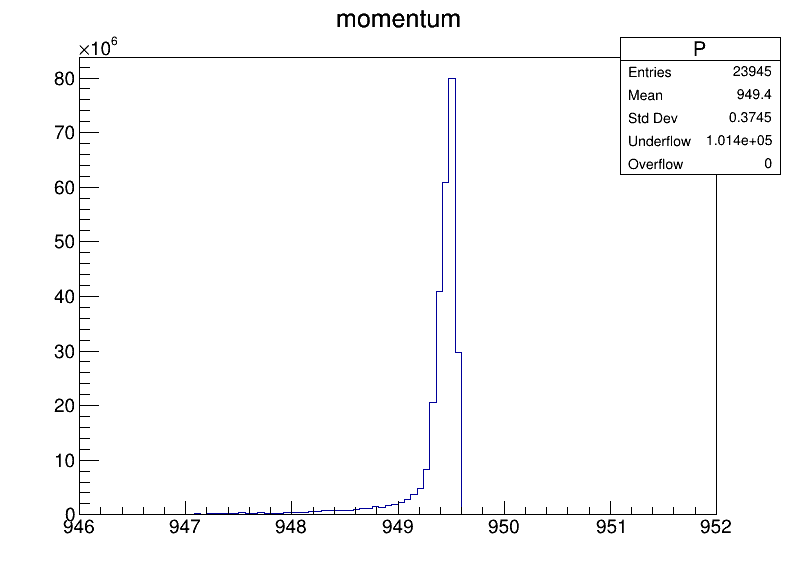
\includegraphics[width=0.5\linewidth]{prex_C_contamination_P}
    \caption{Post target electron momentum distribution. The lower end tail comes 
    from multi-scattering and radiation.}
\end{figure}

The goodness of simulation could be checked by comparison to optics data.
\begin{table}
    \centering
    \begin{tabular}{c c c | c c c c | c c}
	\hline
	\multicolumn{2}{c}{target thickness}	& \multirow{2}{*}{\makecell{p cut \\ (MeV)}}	& \multicolumn{4}{c|}{post target $Q^2$ ($GeV^2$)}   & \multicolumn{2}{c}{Asym ($ppm$)}	\\
	\cline{4-7}
	Pb & C	&   & Pb & C & C (US)	& C (DS) & Pb    & C \\
	\hline
	-5\%	& -5\%	& 2.2	& 0.00625   & 0.00658	& 0.00658   & 0.00658	& 0.55774   & 0.53861 \\
	-5\%	&  0\%	& 2.2	& 0.00626   & 0.00656	& 0.00658   & 0.00654	& 0.55809   & 0.53776 \\
	-5\%	&  5\%	& 2.2	& 0.00627   & 0.00658	& 0.00658   & 0.00657	& 0.55883   & 0.53932 \\
	 0\%	& -5\%	& 2.2	& 0.00627   & 0.00657	& 0.00657   & 0.00657	& 0.55942   & 0.53917 \\
	 0\%	&  0\%	& 2.2	& 0.00626   & 0.00658	& 0.00657   & 0.00660	& 0.55824   & 0.53936 \\
	 0\%	&  5\%	& 2.2	& 0.00627   & 0.00658	& 0.00658   & 0.00658	& 0.55847   & 0.53847 \\
	 5\%	& -5\%	& 2.2	& 0.00625   & 0.00657	& 0.00655   & 0.00658	& 0.55674   & 0.53696 \\
	 5\%	&  0\%	& 2.2	& 0.00627   & 0.00658	& 0.00659   & 0.00657	& 0.55782   & 0.53808 \\
	 5\%	&  5\%	& 2.2	& 0.00629   & 0.00659	& 0.00659   & 0.00659	& 0.55847   & 0.53962 \\
	\hline
	\multicolumn{3}{c|}{average} & 0.00626	& 0.00658   & 0.00658	& 0.00658   & 0.55820   & 0.53859 \\
	\hline
    \end{tabular}
    \caption{Average post target (left arm) $Q^2$ for various thickness configurations. 
    As expected, the $Q^2$ doesn't change with varied foil thicknesses. There is
    some fluctuation in the asymmetry values.}
    % why the C $Q^2$ is a little larger than that of Pb:
    % different scattering angle?
    \label{tab:prex_C_contam_Q2}
\end{table}
From which we can calculate the combined $Q^2$ value
\begin{equation*}
    Q^2 = \frac{R_C Q^2_C + R_{Pb} Q^2_{Pb}}{R_C + R_{Pb}} 
	= \frac{6.71\%\times 0.00658 + 0.00629}{6.71\% + 1} = 0.00629
\end{equation*}

\begin{comment}
\begin{landscape}
    \begin{table}
    \centering
    \begin{tabular}{c c c | c c c c c c c c c c}
	\hline
	\multicolumn{2}{c}{target thicknesses}	& \multirow{2}{*}{\makecell{p cut \\ (MeV)}}	& \multicolumn{2}{c}{$Q^2$ Pb ($GeV^2$)}    & \multicolumn{2}{c}{$Q^2$ C}	& \multicolumn{2}{c}{$Q^2$ C US}  & \multicolumn{2}{c}{$Q^2$ C DS}  & \multicolumn{2}{c}{Asym ($ppm$)}	\\
	Pb & C	&   & vertex	& post vertex	& V	& P-V	& V & P-V   &V	& P-V	& Pb	& C \\
	\hline
	-5\%	& -5\%	& 2.2	& 0.00608   & 0.00625   & 0.00649   & 0.00658	& 0.00641   & 0.00658	& 0.00658   & 0.00658	& 0.55774   & 0.53861 \\
	-5\%	&  0\%	& 2.2	& 0.00609   & 0.00626   & 0.00648   & 0.00656	& 0.00643   & 0.00658	& 0.00654   & 0.00654	& 0.55809   & 0.53776 \\
	-5\%	&  5\%	& 2.2	& 0.00610   & 0.00627   & 0.00650   & 0.00658	& 0.00643   & 0.00658	& 0.00657   & 0.00657	& 0.55883   & 0.53932 \\
	 0\%	& -5\%	& 2.2	& 0.00611   & 0.00627   & 0.00650   & 0.00657	& 0.00643   & 0.00657	& 0.00657   & 0.00657	& 0.55942   & 0.53917 \\
	 0\%	&  0\%	& 2.2	& 0.00609   & 0.00626   & 0.00650   & 0.00658	& 0.00641   & 0.00657	& 0.00660   & 0.00660	& 0.55824   & 0.53936 \\
	 0\%	&  5\%	& 2.2	& 0.00610   & 0.00627   & 0.00649   & 0.00658	& 0.00641   & 0.00658	& 0.00658   & 0.00658	& 0.55847   & 0.53847 \\
	 5\%	& -5\%	& 2.2	& 0.00607   & 0.00625   & 0.00647   & 0.00657	& 0.00637   & 0.00655	& 0.00658   & 0.00658	& 0.55674   & 0.53696 \\
	 5\%	&  0\%	& 2.2	& 0.00609   & 0.00627   & 0.00649   & 0.00658	& 0.00641   & 0.00659	& 0.00657   & 0.00657	& 0.55782   & 0.53808 \\
	 5\%	&  5\%	& 2.2	& 0.00610   & 0.00629   & 0.00650   & 0.00659	& 0.00643   & 0.00659	& 0.00659   & 0.00659	& 0.55847   & 0.53962 \\
	\hline
	\multicolumn{3}{c}{average} &0.00609 & 0.00626	& 0.00649   & 0.00658	& 0.00642   & 0.00658	& 0.00658   & 0.00658	& 0.55820   & 0.53859 \\
    \end{tabular}
	\caption{Average $Q^2$}
    \end{table}
\end{landscape}

I am doubting if I was comparing the same thing. 
In data, $Q^2$ was calculated as:
$$ Q^2 = 2*beamE*P*(1-\cos(\theta))$$
where beamE was the average beam energy (before hitting the target), 
and P was the reconstructed beam energy, or post-target energy 
and $\theta$ was the reconstructed scattering angle 

But in simulation, $Q^2$ was calculated as:
$$ Q^2 = 2*E*Ef*(1-\cos(\theta)) $$
where E was the post vertex beam energy: I made a mistake here, E should be 
pre-vertex beam energy.
$$ Ef = M*E/(M + E*(1-cos(th))) $$
was the theorectical beam energy after elastic scattering and $\theta$ was 
the scattering angle.

Obviously, data and simulation had different definitions:
$$ beamE > E	\quad P < E	\quad P \stacker{?}{\sim} $$
The only good news was that beamE, E, P, Ef were all close to each other. Overall,
the simulation would make the simulation $Q^2$ smaller than that of data. Not
sure how large the uncertainty was.

The only difference here for vertex and post-vertex was the scattering angle,
one was the vertex angle and the other being the post-target scattering angle.

The CREX analysis was comparing the same thing.
\end{comment}

Compare the simulation $Q^2$ to optics data. We saw quite good agreement in left
arm. For the right arm, the larger scattering angle caused a little difference
in $Q^2$ (2\%).
\begin{table}
    \centering
    \begin{tabular}{c | c c}
	\hline
	arm & $\theta$	& $Q^2$ ($GeV^2$)   \\
	\hline
	Left	& $4.748 \pm 0.006$ & $0.00627 \pm 0.00002$	\\
	Right	& $4.813 \pm 0.004$ & $0.00642 \pm 0.00001$	\\
	\hline
    \end{tabular}
    \caption{Average $\theta$ and $Q^2$ for left and right arms. These values were
    combination of Pb and C.}
    \label{tab:prex_C_contam_Q2}
\end{table}

To study the systematic uncertainties, we varied the thickness of \Pb foil and 
diamond foil (total thickness) by 5 percent based on the nominal values, and applied
different momentum cut (varied from 1.8 to 2.6 $MeV$), the result is shown in
Table~\ref{tab:prex_C_contam_rate_thickness} and \ref{tab:prex_C_contam_rate_pcut}. 
$f_c$ is the rate fraction.
\begin{table}[h!]
    \centering
    \begin{tabular}{=c +c | c | +c +c +c +c}
	\hline
	\makecell{\Pb thickness \\ variation}	& \makecell{C thickness	\\ variation}	
	& \makecell{p cut \\ (MeV)} & \makecell{C rate \\ (MHz)}    & \makecell{\Pb rate \\ (MHz)}  
	& $\frac{R_C}{R_{Pb}} (\%)$	& $f_c = \frac{R_C}{R_C + R_{Pb}}$ (\%)	\\
	\hline
	-5\% & -5\% &	  & 1.26E+2 & 1.88E+3 & 6.72 & 6.30	\\
	-5\% &  0\% &     & 1.34E+2 & 1.90E+3 & 7.05 & 6.59   \\
	-5\% &  5\% &     & 1.38E+2 & 1.90E+3 & 7.23 & 6.75   \\
	 0\% & -5\% &     & 1.22E+2 & 1.90E+3 & 6.43 & 6.04   \\
	 \rowstyle{\color{red}}   
	 0\% &  0\% & 2.2 & 1.29E+2 & 1.93E+3 & 6.71 & 6.29   \\
	 0\% &  5\% &     & 1.35E+2 & 1.89E+3 & 7.11 & 6.64   \\
	 5\% & -5\% &     & 1.16E+2 & 1.95E+3 & 5.94 & 5.61   \\
	 5\% &  0\% &     & 1.22E+2 & 1.94E+3 & 6.31 & 5.93   \\
	 5\% &  5\% &     & 1.28E+2 & 1.91E+3 & 6.72 & 6.30   \\
	\hline
    \end{tabular}
    \caption{Scattering rate of the \Pb and diamond foils with different foil
    thicknesses.}
    \label{tab:prex_C_contam_rate_thickness}
\end{table}

\begin{table}[h!]
    \centering
    \begin{tabular}{=c c | +c | +c +c +c +c}
	\hline
	\makecell{\Pb thickness \\ variation}	& \makecell{C thickness	\\ variation}	
	& \makecell{p cut \\ (MeV)} & \makecell{C rate \\ (MHz)}    & \makecell{\Pb rate \\ (MHz)}  
	& $\frac{R_C}{R_{Pb}} (\%)$	& $f_c$ (\%)	\\
	\hline
	\multirow{12}{*}{0\%}	& \multirow{12}{*}{0\%}	&
	    1.80 & 1.24E+2 & 1.86E+3 & 6.68 & 6.26  \\
	& & 1.90 & 1.25E+2 & 1.87E+3 & 6.69 & 6.27  \\
	& & 2.00 & 1.27E+2 & 1.89E+3 & 6.70 & 6.28  \\
	& & 2.05 & 1.27E+2 & 1.90E+3 & 6.70 & 6.28  \\
	& & 2.10 & 1.28E+2 & 1.91E+3 & 6.71 & 6.28  \\
	& & 2.15 & 1.29E+2 & 1.92E+3 & 6.71 & 6.29  \\
	\rowstyle{\color{red}}   
	& & 2.20 & 1.29E+2 & 1.93E+3 & 6.71 & 6.29  \\
	& & 2.25 & 1.30E+2 & 1.94E+3 & 6.72 & 6.30  \\
	& & 2.30 & 1.31E+2 & 1.95E+3 & 6.73 & 6.30  \\
	& & 2.35 & 1.31E+2 & 1.95E+3 & 6.73 & 6.31  \\
	& & 2.40 & 1.32E+2 & 1.96E+3 & 6.74 & 6.32  \\
	& & 2.60 & 1.34E+2 & 1.99E+3 & 6.74 & 6.32  \\
	\hline
    \end{tabular}
    \caption{Scattering rate of the \Pb and diamond foils with different momentum 
    cut.}
    \label{tab:prex_C_contam_rate_pcut}
\end{table}

The uncertainty for each variation was taken to be the absolute difference 
from the nominal value, as shown below:
\begin{table}
    \centering
    \begin{tabular}{c | c c | c c}
	\hline
	variation   & maximum	& diff in $f_C$  & minimum    & diff in $f_C$ \\
	\hline
	Pb & (-5, 0) - (0, 0)	& 2.98E-3   & (+5, 0) - (0, 0)	& -3.55E-3  \\
	C  & (0, +5) - (0, 0)	& 3.53E-3   & (0, -5) - (0, 0)	& -2.49E-3  \\
	p cut	& (2.6) - (2.2)	& 2.93E-4   & (1.8) - (2.2)	& -2.88E-4  \\
	\hline
	total	&   & 4.63E-3	&   & 4.35E-3	\\
	\hline
    \end{tabular}
    \caption{The maximum and minimum difference for each variation. (n1, n2) 
    represents the configuration of target foils' thicknesses. n1 for Pb foil
    and n2 for C foil. (pcut) indicates the p cut value}
    \label{tab:prex_C_contam_error}
\end{table}
Based on Table~\ref{tab:prex_C_contam_error}, a conservative error value 
(the larger one) was used , which gave out the final value of $f_C$
\begin{equation*}
    f_C = 0.0629 \pm 0.005
\end{equation*}

%%%%%%%%%%%%%%%%%%%%%%%%
\subsubsection{Cross Check}
The scattering rate is proportional to the cross section and number of atoms
in unit area. 
\begin{equation}
    R \propto \sigma \times N = \sigma \times \frac{t}{m}
\end{equation}
t and m are, respectively, area density and atomic mass. Therefore
\begin{equation}
    \frac{R_C}{R_{Pb}} = \frac{\sigma_C}{\sigma_{Pb}} \times \frac{t_c}{t_{Pb}} \times \frac{m_{Pb}}{m_C}
\end{equation}
Take $E = 0.95\ GeV$ and $\theta = 4.8^\circ$ (based on Table~\ref{tab:prex_C_contam_Q2}), 
our theorist friends predicted the cross section of C and Pb to be
\begin{equation*}
    \sigma_C = 48.001\ mbarn	\qquad \sigma_{Pb} = 3386.100\ mbarn	
\end{equation*}
% this angle is different from what we used in simulation 4.74

The ratio of $t_C/T_{Pb}$ was calculated as
\begin{table}[!h]
    \centering
    \begin{tabular}{c | c c c | c c c}
	\hline
	target	& \makecell{$t_C$ (US + DS) \\ ($mg/cm^2$)} & \makecell{$t_{Pb}$ \\ ($mg/cm^2$)}	
	& $t_C/t_{Pb}$  & \makecell{main detector \\ error n} & \makecell{weight \\ $1/\sqrt{n}$}    & \makecell{weighted \\ $t_C/t_{Pb}$} \\
	\hline
	Pb208\#2    & 177.6	& 632	& 0.281	& 42.743    & 0.1530	& 0.037 \\
	Pb208\#10   & 180	& 623	& 0.289	& 33.3465   & 0.1732	& 0.043	\\
	Pb208\#9    & 180	& 615   & 0.293 & 28.9264   & 0.1859   	& 0.047	\\
	Pb208\#8    & 180	& 620   & 0.290 & 33.5835   & 0.1726   	& 0.043	\\
	Pb208\#5    & 176.8	& 632   & 0.280 & 36.3435   & 0.1659   	& 0.040	\\
	Pb208\#7    & 180	& 639   & 0.282 & 32.7936   & 0.1746   	& 0.042	\\
	Pb208\#6    & 180	& 618   & 0.291 & 47.6238   & 0.1449   	& 0.036	\\
	\hline
		    & 179.2	& 625.6	& 0.286	&	    & 1.1700	& \color{red} 0.287 \\
	\hline                                                
    \end{tabular}
    \caption{Calculation of weighted $t_C/T_{Pb}$, the main detector error was
    the uncertainty of the main detector mean value (reg\_asym\_us\_avg); the 
    weighted ratio was calculated as $\frac{w_j}{\sum_i w_i} \times \left( t_C/t_{Pb} \right)_j$.}
    \label{tab:ratio_of_area_density}
\end{table}

\begin{table}[!h]
    \centering
    \begin{tabular}{c c | c c c | c c}
	\hline
	E ($GeV$)   & $\theta$  & Target    & $\sigma$ ($mbarn$)    & m & $\frac{R_C}{R_{Pb}}$ (\%) & $f_C$ (\%)    \\
	\hline
	\multirow{2}{*}{0.95}	& \multirow{2}{*}{$4.8^\circ$}	& 
	      \C    & 48.001	& 12.011    & \multirow{2}{*}{7.04} & \multirow{2}{*}{6.57} \\
	\cline{3-5}
	&   & \Pb   & 3386.100	& 207.977   &	& \\
	\hline
    \end{tabular}
    \caption{Theoretical calculation of $f_C$. These are updated values. In the 
    initial study, the scattering angle was chosen to be $4.8^\circ$, with corresponding
    $\sigma_C = 48.001\ mbarn$ and $\sigma_{Pb} = 3386.1\ mbarn$, leading to
    $R_C/R_{Pb} = 7.04\%$ and $f_C = 6.57\%$.}
\end{table}
The theoretical value was 4.6\% higher than the simulation result.

\subsubsection{Contribution to $\CA_{pv}$}
As said before, the asymmetry from carbon scattering was well understood, and
we had a table of cross section and asymmetry for electron-carbon elastic scattering
at various energies and scattering angles, which were numerical solved from the Dirac equation
by our theoretical friends. The same for Pb.
The asymmetry for carbon was taken to be $539.36 \ ppb$ as shown in Table~\ref{tab:prex_C_contam_Q2}
with the nominal Pb and nominal C thicknesses. The uncertainty for it was taken
to be a conservative estimation of 4\%.
\begin{figure}
    \centering
    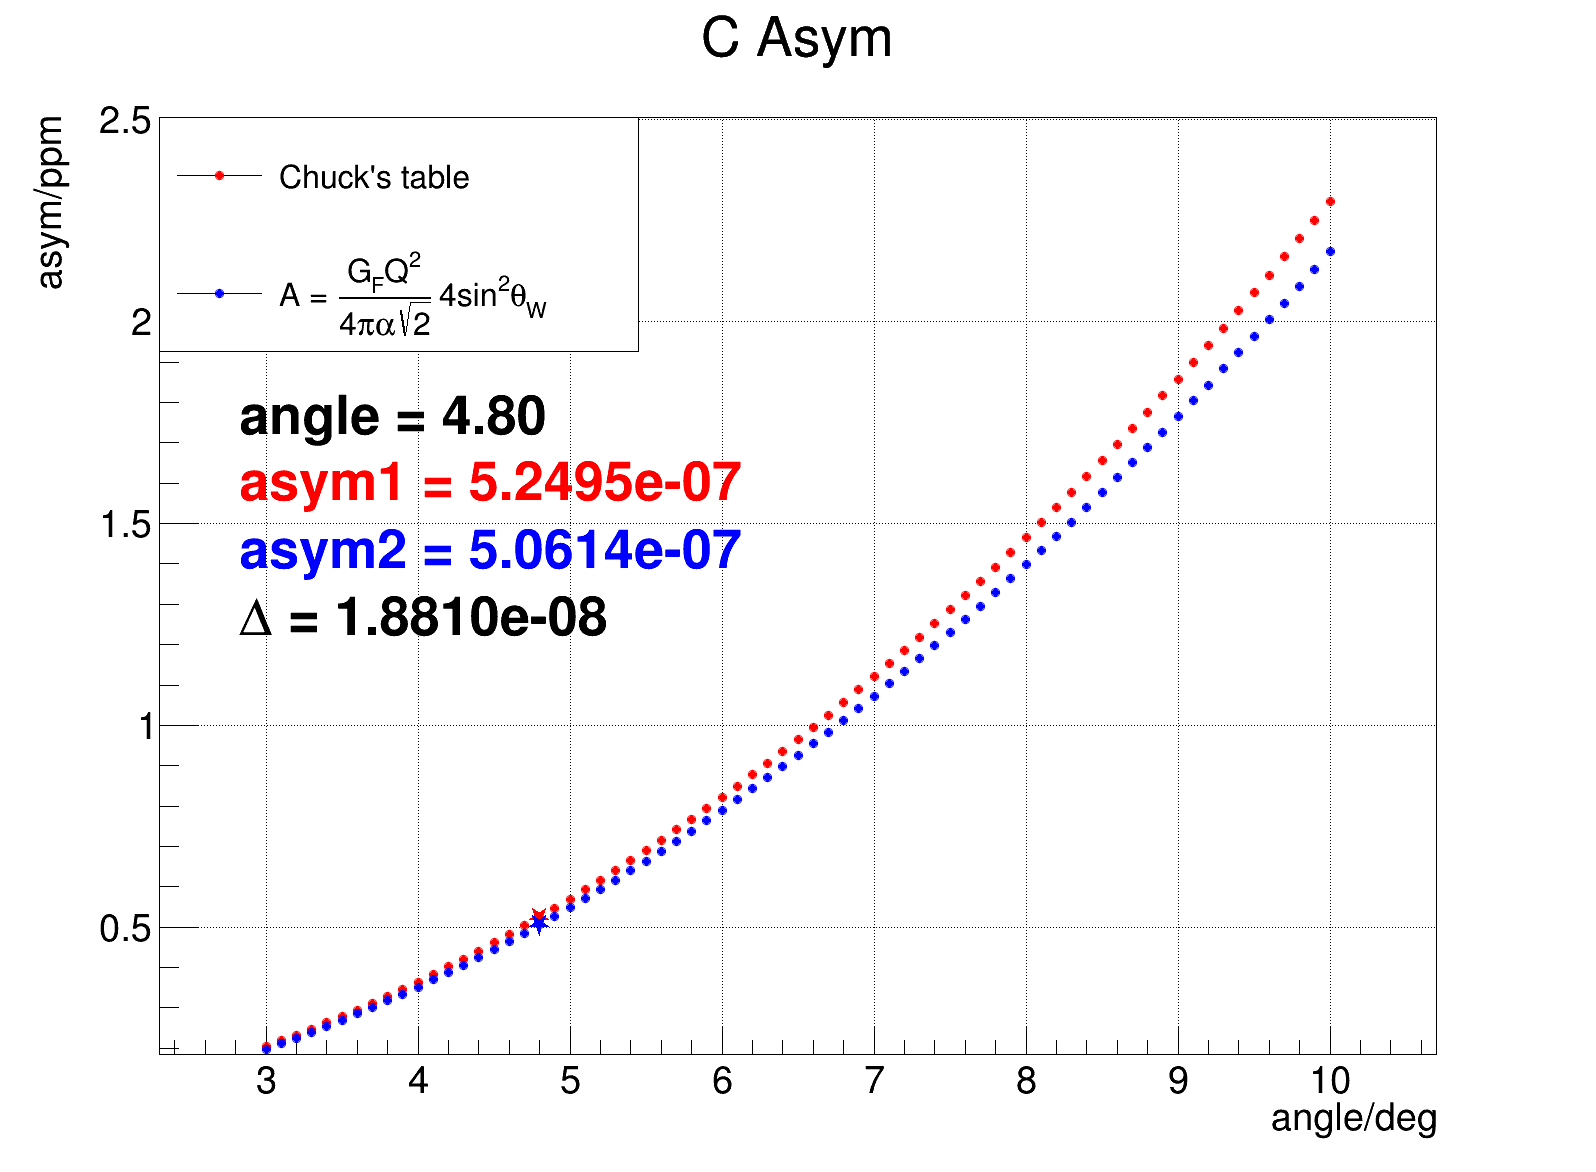
\includegraphics[width=0.49\linewidth]{prex_asym_C}
    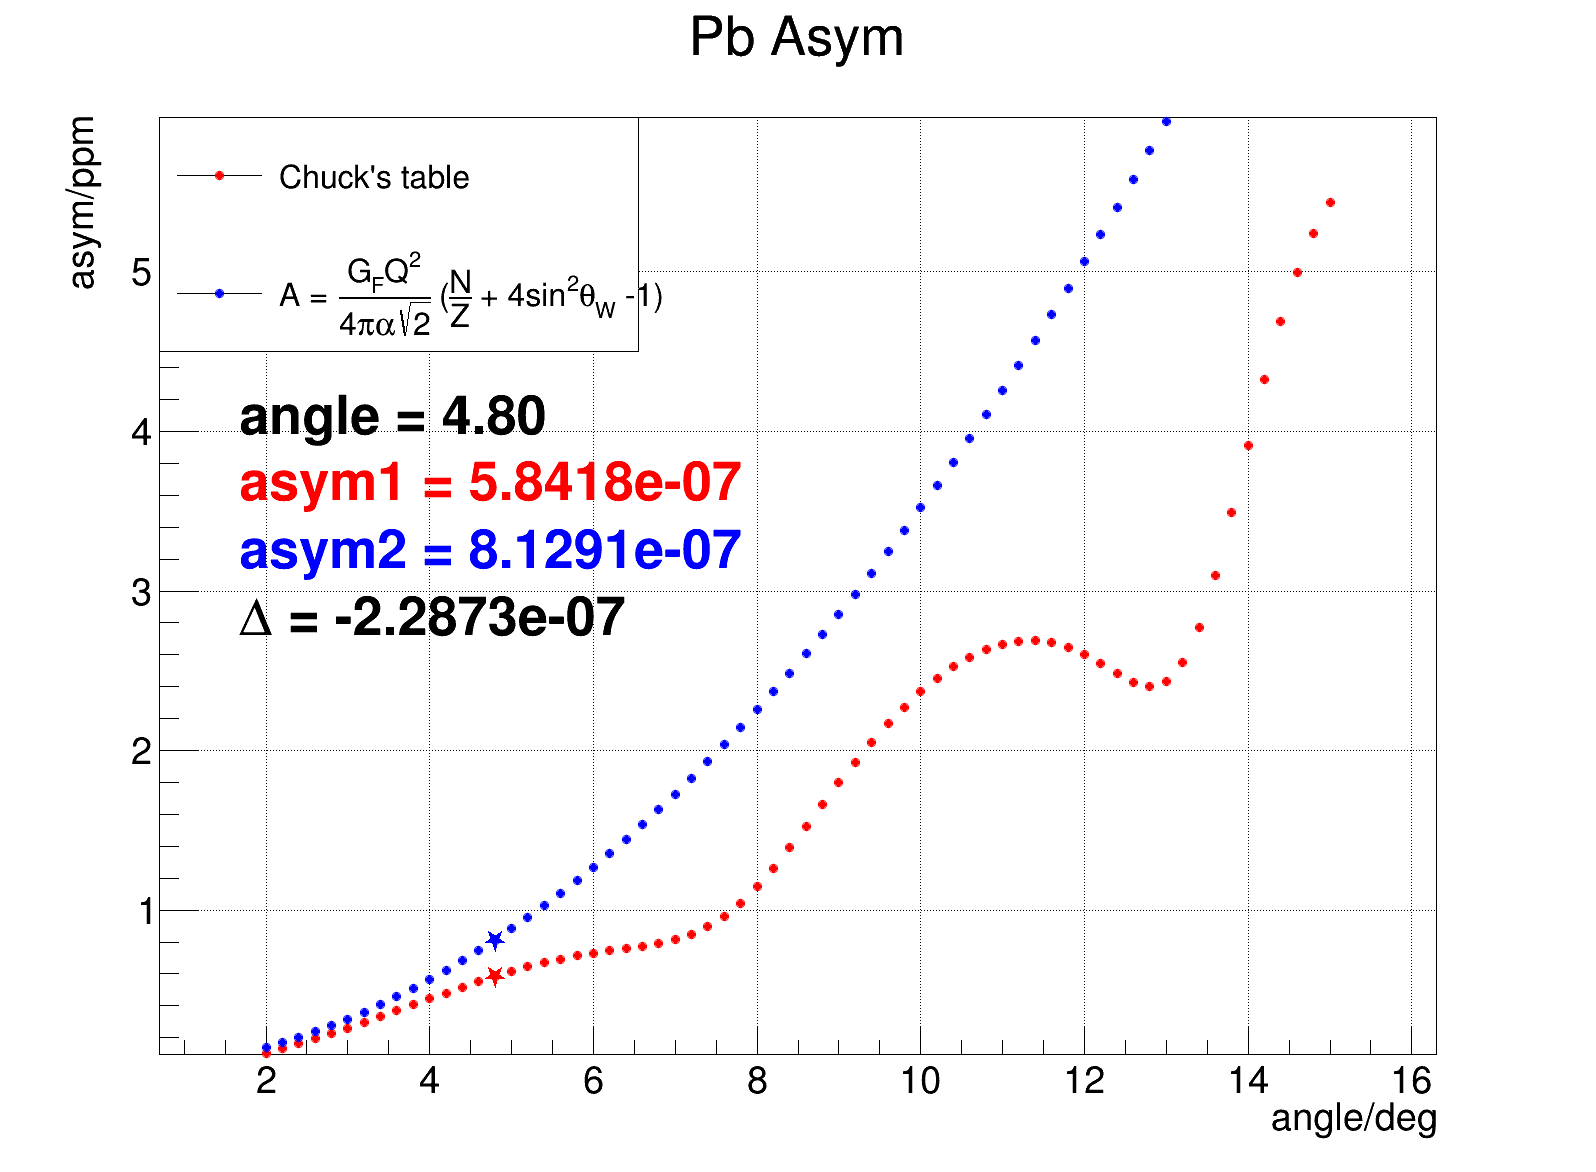
\includegraphics[width=0.49\linewidth]{prex_asym_Pb}
    \caption{Theoretical values of the asymmetry for C and Pb in our experimental 
    dynamics predicted by Chuck's table, which included Coulomb correction, cross
    checked with a Standard Model Born approximation calculation. We see similar
    asymmetry values for C and Pb.}
    \label{prex_asym}
\end{figure}
Using Eq.~\ref{eq:systematic_uncertainty}, we could calculate the uncertainty
contribution to $\CA_{pv}$, summarized in Table~\ref{tab:prex_C_contam}
\begin{equation*}
    \begin{gathered}
	\frac{\partial \CA_{pv}}{\partial \CA_C} \delta \CA_C = 
	-\frac{0.0629}{1 - 0.0629} \times 4\% \times 539.36 = -1.4481\ ppb   \\
	\frac{\partial \CA_{pv}}{\partial f_C}\delta f_C =
	\frac{550 - 539.46}{1 - 0.0629} \times 0.00463 = 0.0521\ ppb	\\
    \end{gathered}
\end{equation*}

\begin{table}
    \centering
    \begin{tabular}{c | c c | c c | c c}
        \hline
	\thead{$\CA_{cor}/\CP$ \\ ($ppb$)}   & \thead{$\CA_C$ \\ ($ppb$)}   & $\frac{\delta\CA_C}{\CA_C}$   & $f_C$ & $\delta f_C$  & \thead{rel. error \\ due to $\CA_C$ } & \thead{rel. error \\ due to $f_C$}\\
        \hline
	549.34	& $539.36$  & 4\%   & 6.29\%	& 0.463\%   & 0.26\%	& 0.01\% \\
        \hline
    \end{tabular}
    \caption{Relative uncertainty due to $\CA_C$ and $f_C$.}
    \label{tab:prex_C_contan}
\end{table}
The uncertainty caused by error in $f_C$ was negligible, and the one from $\CA_C$
was also tiny, which in hindsight, justifies our adoption of the sandwich target.

\begin{comment}
% somehow, the rate derivation was wrong
\bigskip
One could also estimate the rate from measurement. 
\begin{eqaution}
    \sigma = \sqrt{\frac{1}{R/30}}
\end{eqaution}
\begin{table}[!h]
    \centering
    \begin{tabular}{c c c | c c c c c c}
	\hline
	Target	& run	& I $(\mu A)$   & \thead{rms \\ ($ppm$)} & \thead{rms@$70\ \mu A$ \\ ($ppm$)} & \thead{bcm res. \\ ($ppm$)}   & \thead{bpm res. \\ ($ppm$)}   & \thead{cor. rms \\ ($ppm$)}  & \thead{rate \\ ($GHz$)}  \\
	\hline
	C12	& 4133	& 86.2	& 143	& 158.7	& 20	& 25	& 150.4	& 1.326	\\
	D-Pb-D	& 4112	& 67.7	& 93	& 91.5	& 20	& 25	& 82.9	& 4.365	\\
	\hline
    \end{tabular}
    \caption{The corrected rms was calculated as: $\sqrt{\frac{\sigma^2 - \sigma^2_{bcm} - \sigma^2_{bpm}}{1 + 0.26^2}}$}
% why the factor of 0.26
\end{table}
The C graphite target has a thickness of $1.991\ mm$ and a density of 
\end{comment}


%%%%%%%%%%%%%%%%%%%%%%%%%%%%%%%%%%%%%%%%%%%%%%%%%%%%%%%%%%%%%%%%%%%%%%%%
\section{Acceptance Function}
As we said before, the spectrometer acceptance was mainly defined by the Q1 
collimator, but other devices may also have affections on it. And the accepted
area was not tiny ($0.00377 \ sr$), not every point within the acceptance had
the same detection efficiency and cross section asymmetry, therefore what
we measured was actually the average asymmetry over the acceptance:
\begin{equation}
    \CA_{mea} = \frac{\int d\theta \sin\theta A(\theta) \frac{d\sigma}{d\Omega} \epsilon(\theta)}{\int d\theta \sin\theta \frac{d\sigma}{d\Omega} \epsilon(\theta)}
    \label{eq:acceptance_function}
\end{equation}
Here $\epsilon(\theta)$ is the acceptance function, which is defined as
the ratio of electrons that reach the main detector over all scattered
electrons, which depends on the scattering angle $\theta$:
\begin{equation}
    \epsilon(\theta) = \frac{N_{det}(\theta)}{N_{sca}}
    \label{eq:acceptance_definition}
\end{equation}

From Eq.~\ref{eq:acceptance_function}, we see the importance of the acceptance
function. Firstly, it will be a systematic uncertainty of our asymmetry
measurement; and secondly, only with the acceptance function, can we compare
our experimental measurement to theoretical predictions to interpret our
result.

To extract the acceptance function, we had to turn to simulation. Then how
did we know our simulation was correct? We will compare the simulation result
to optics data, and precise match of various kinematic variables between simulation
and data was required. 

When we took optics data, we would put in the sieve slit collimators so that 
we could reconstruct electron trajectory using track info from VDCs 
to match holes in the sieve plane, therefore we could know the scattering angle and 
energy for each electron trajectory.

In terms of simulation, we tuned a few parameters to find out the best
match: so called the best model, which was then used to calculate the acceptance
function. The few parameters we explored were:
\begin{itemize}
    \item Septum current
    \item Q1 collimator shift
    \item Pinch point shift
\end{itemize}

%%%%%%%%%%%%%%%%%%%%%%%%%%%%%%%%%%%%%%%%%%%%%%%%
\subsection{Transportation Matrix}
Due to the existence of various magnetic fields (septum, HRS) from target to detector, 
there is no way to know the exact analytical expression of the transportation
from target to detector, though we can approximate and measure it.

The electron's trajectory can be parameterized as: $\vec{X} = (x, \theta, y, \phi, \delta)^T$ 
w.r.t. to a reference trajectory (usually the central ray). In the transport coordinate, 
$\hat{z}$ is the direction of reference trajectory;
x is the displacement in the dispersive plane relative to the reference 
trajectory, and $\theta$ is electron's `velocity' in the dispersive plane:
$\theta = \frac{\partial x}{\partial z}$; similarly, y and $\phi$ are displacement
and `velocity' in the y-z plane, $\hat{y}$ is oriented such that $\hat{x}$, 
$\hat{y}$, $\hat{z}$ are orthogonal to each other and they form a 
right-handed coordinate $\hat{z} = \hat{x} \times \hat{y}$.
$\delta = \frac{\Delta p}{p}$ represents the fractional deviation of momentum
from that of the reference trajectory. With these definitions, we can expressed
one electron's position along the optical path as a Fourier expansion of the
initial position of $\vec{X}_0$
\begin{equation}
    x_i = \sum_j T_{ij} x_{j,0} + \sum_j \sum_k S_{ijk} x_{j,0}x_{k, 0} + \cdots
\end{equation}
$T_{ij}$ is what we call the transportation matrix, whose elements indicate
the reliance of beam position parameters on each other: $T_{ij} = \frac{\partial x_i}{\partial x_j}$.
First order is a good approximation of the transportation formula. So that we
have:
\begin{equation}
    \begin{pmatrix}
	x   \\
	y   \\
	\theta	\\
	\phi	\\
	\delta	\\
    \end{pmatrix}
    =
    T
    \begin{pmatrix}
	x_{tg}   \\
	y_{tg}   \\
	\theta_{tg}	\\
	\phi_{tg}	\\
	\delta_{tg}	\\
    \end{pmatrix}
    =
    \begin{pmatrix}
	x|x_{tg} & x|y_{tg}   & x|\theta_{tg}	& x|\phi_{tg}    & x|\delta_{tg}    \\
	y|x_{tg} & y|y_{tg}   & y|\theta_{tg}	& y|\phi_{tg}    & y|\delta_{tg}    \\
	\theta|x_{tg} & \theta|y_{tg}   & \theta|\theta_{tg}	& \theta|\phi_{tg}    & \theta|\delta_{tg}    \\
	\phi|x_{tg} & \phi|y_{tg}   & \phi|\theta_{tg}	& \phi|\phi_{tg}    & \phi|\delta_{tg}    \\
	\delta|x_{tg} & \delta|y_{tg}   & \delta|\theta_{tg}	& \delta|\phi_{tg}    & \delta|\delta_{tg}    \\
    \end{pmatrix}
    \begin{pmatrix}
	x_{tg}   \\
	y_{tg}   \\
	\theta_{tg}	\\
	\phi_{tg}	\\
	\delta_{tg}	\\
    \end{pmatrix}
\end{equation}
The `tg' subscript means corresponding values at the target plane. With this matrix, we can
propagate backward (inverse of T) to calculate electron position at the exit 
of the target from what we detect using VDCs. Usually we calculate the beam
position on the focal plane $\vec{X}_{fp}$, then the beam position on the target
plane will be: 
\begin{equation}
    \vec{X}_{tg} = T^{-1} \vec{X}_{fp}
    \label{eq:reconstruction}
\end{equation}
The reason that we don't use BPM to `measure' beam position/angle on target is that 
multi-scattering/radiation inside the target foil will distort the beam trajectory. 

A typical HRS transportation plot looks like Fig. \ref{fig:hrs_transport}:
\begin{figure}[H]
    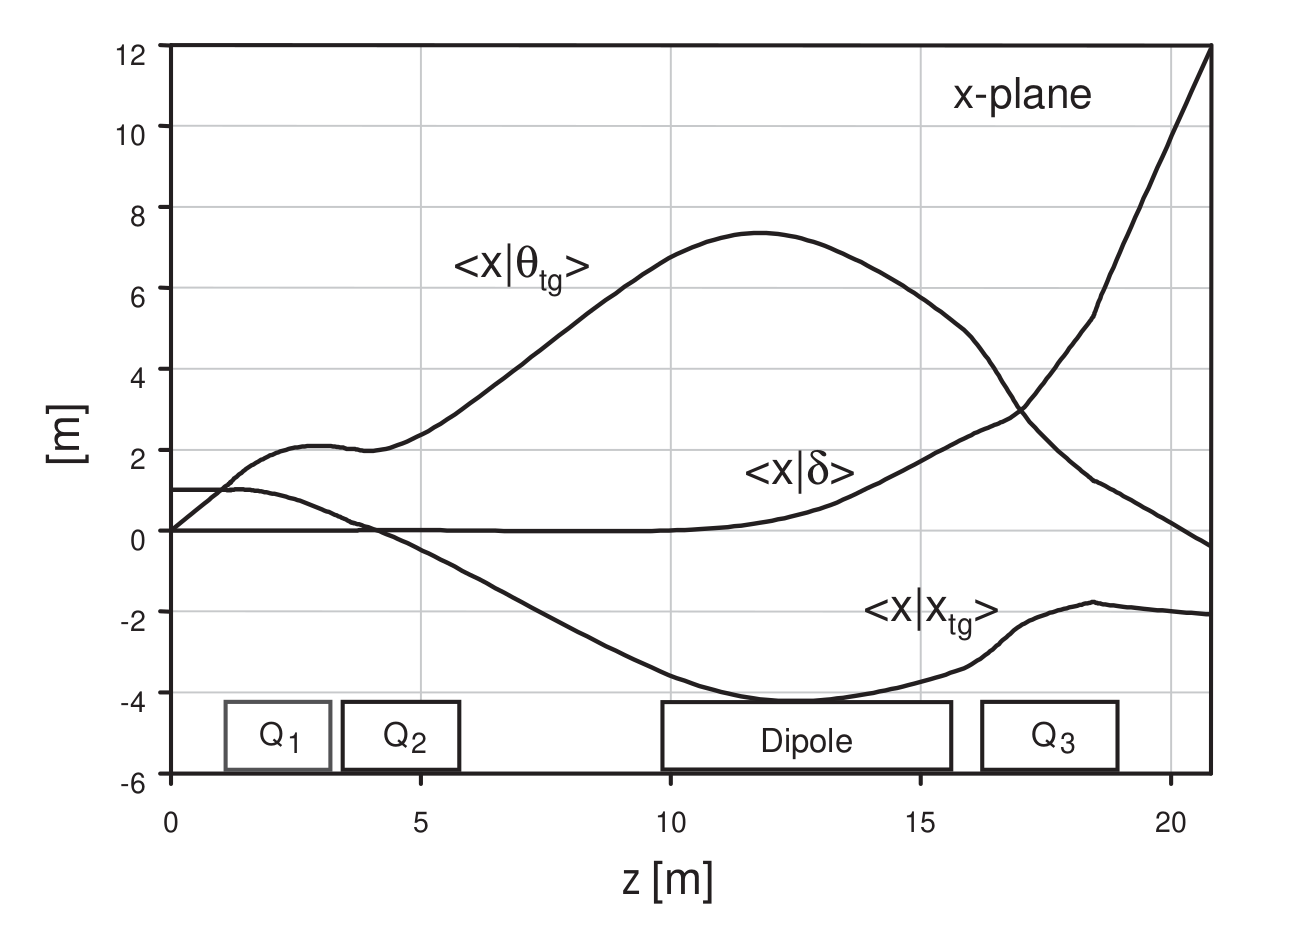
\includegraphics[width=0.50\linewidth]{hrs_transport_x}
    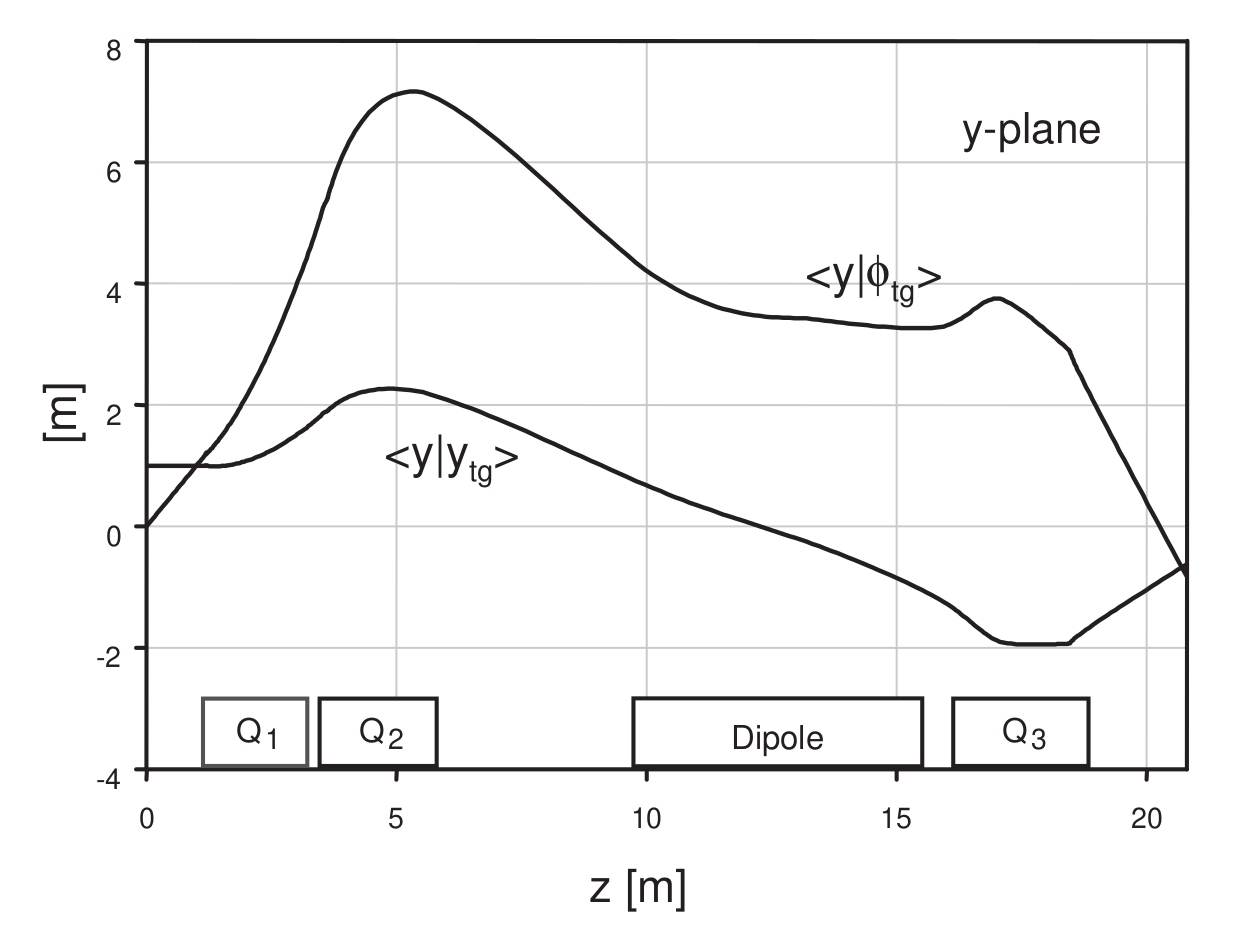
\includegraphics[width=0.48\linewidth]{hrs_transport_y}
    \caption{Transportation plot of HRS. One can clearly see the dispersion effect
    due to shift in momentum ($\delta$) in the Dipole area and the convergent effect
    of Q3.}
    \label{fig:hrs_transport}
\end{figure}

Actually, we don't need to measure every element of T, some elements are obviously
0. E.x. $\delta$ should be not be changed by any magnetic field, so $T_{5i, i\ne 5} = 0$.
The design of HRS tells us that the dispersion depends only on $\delta$, but not
on $\theta$ or $\phi$, so $x|\theta = 0$. Different planes should not
interfere with each other, so that $x|y = x|\phi = \theta|y = \theta|\phi 
= y|x = y|\theta = \phi|x = \phi|\theta = 0$. This is a sparse matrix.

The matrix elements were measured using beam trajectory with sieve slit collimator
inserted in. When the sieve slit collimator was put in, the electron trajectory
from different holes were naturally separated on the focal plane, which allowed
us to match them to sieve holes one by one. With a reasonable initial value of 
the transportation matrix (from previous experiments),
we could reconstruct electron's trajectory on the sieve plane using Eq.~\ref{eq:reconstruction}.
By tuning the matrix element, the one that minimizes the distance of each electron's trajectory on the sieve
plane from its corresponding hole center was identified as the transportation
matrix, so this is a linear regression problem. The identification of the septum 
and HRS current was based on the sieve pattern calculated from the 
transportation matrix. 

% The transportation matrix was extracted for following optics runs:
% \begin{table}
%     \centering
% \end{table}
% what's the difference between PREX-II and CREX?
% how many non-zero elements on the initial matrix?
% which run was used? how different runs/number of effects affect the final result
% energy on the quartz plane:

%%%%%%%%%%%%%%%%%%%%%%%%%%%%%%%%%%%%%%%%%%%%%%%%
\subsection{Scattering Angle $\theta_{lab}$}
The parameter that directly reflects the quality of simulation is the scattering
angle, while it was more convenient to use the Target Coordinate System (TCS) 
than the Hall Coordinate System (HCS) in simulation, we finally were comparing
the scattering angle in the lab frame. The 2 coordinate systems and the transportation
between them are defined below.

\begin{itemize}
    \item Hall Coordinate System: originated at the center of the hall and
	cross the beam line.  $\hat{Z}$ is along the beam line, pointing downstream; 
	$\hat{y}$ points up and $\hat{x}$ points left to form a RH coordinate system.
    \item Target Coordinate System: each HRS specific, the transport coordinate at target position.
	$\hat{z}$ is along the beam trajectory, pointing away the target, 
	$\hat{x}$ in the dispersive plane and points down, $\hat{y}$ is perpendicular
	to the dispersive plane and points away (toward) the beamline for L-HRS (R-HRS).
\end{itemize}

\begin{figure}[H]
    \begin{subfigure}[b]{0.5\textwidth}
	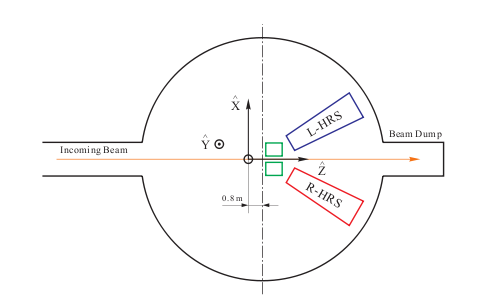
\includegraphics[width=\linewidth]{HCS}
	\caption{Top view of HCS}
    \end{subfigure}
    \begin{subfigure}[b]{0.5\textwidth}
	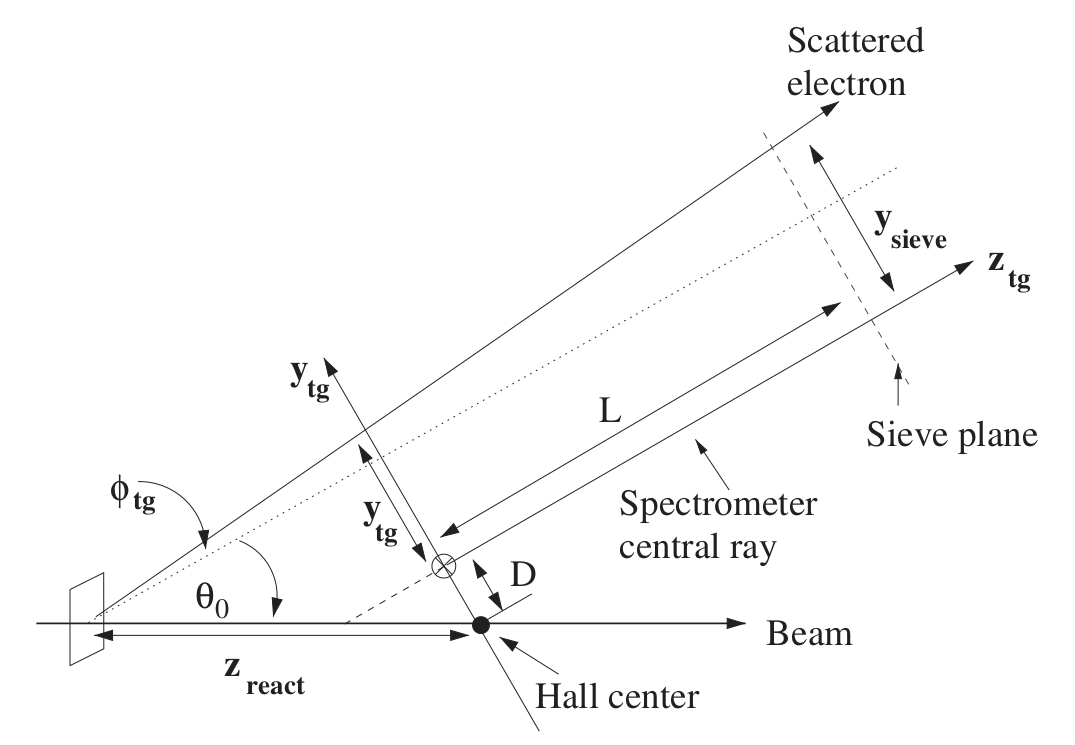
\includegraphics[width=\linewidth]{TCS}
	\caption{Top view of TCS}
    \end{subfigure}
    \caption{Schematic plot of HCS and TCS. The Hall center is the origin of the 
    HCS, but the target doesn't necessary lie in the Hall center. The distance
    from the Hall center to the sieve plane L is constant, which is used to
    identify the origin of the TCS. In ideal case, the origins of both coordinate
    systems will overlap.}
\end{figure}

The relationship between HCS and TCS is:
\begin{equation}
    \begin{pmatrix}
	x_{tg}	\\
	y_{tg}	\\
	z_{tg}	\\
    \end{pmatrix}
    =
    \begin{pmatrix}
	\cos(90^\circ)   & -\sin(90^\circ)    & 0	\\
	\sin(90^\circ)   & \cos(90^\circ)     & 0	\\
	0   & 0     & 1	\\
    \end{pmatrix}
    \begin{pmatrix}
	\cos(-\theta_0)	& 0 & -\sin(-\theta_0)  \\
	0		& 1 & 0		\\
	\sin(-\theta_0)	& 0 & \cos(-\theta_0)  \\
    \end{pmatrix}
    \begin{pmatrix}
	x   \\
	y   \\
	z   \\
    \end{pmatrix}
\end{equation}

\begin{equation}
    \left.
    \begin{aligned}
	x_{tg}	&= -y	\\
	y_{tg}	&= x\cos\theta_0 + z\sin\theta_0    \\
	z_{tg}	&= -x\sin\theta_0 + z\cos\theta_0   \\
    \end{aligned}
    \right\}
    \iff
    \left\{
    \begin{aligned}
	x   &= y_{tg}\cos\theta_0 + z_{tg}\sin\theta_0	\\
	y   &= -x_{tg}	\\
	z   &= -y_{tg}\sin\theta_0 + z_{tg}\cos\theta_0   \\
    \end{aligned}
    \right.
\end{equation}
Define $R = \left(x^2 + y^2 + z^2\right)^{1/2} = z_{tg} \left(\phi^2_{tg} + \theta^2_{tg} + 1\right)^{1/2}$.
So the scattering angle in the lab frame will be:
\begin{equation}
    \cos\theta = \frac{z}{R} = \frac{-\phi_{tg}\sin\theta_0 + \cos\theta_0}{\left(\phi^2_{tg} + \theta^2_{tg} + 1\right)^{1/2}}
\end{equation}
For data, $\theta_0$ was identified to be $4.789^\circ$ ($4.771^\circ$) for
L-HRS (R-HRS). In simulation, both arms used $4.74^\circ$. Note that $\theta_{lab}$
is a post-target (apparent) quantity, which includes effect of post-vertex radiation and
multi-scattering, not the `real' scattering angle (vertex quantity) at the vertex 
where the interesting PV elastic scattering happens. The correction from the apparent 
distribution to the vertex distribution is about 1.5\%.
\begin{figure}[H]
    \centering
    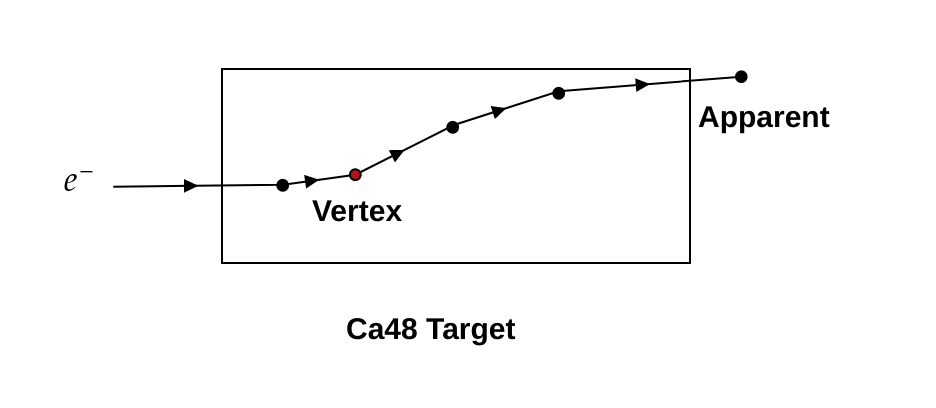
\includegraphics[width=0.5\linewidth]{scattering}
    \caption{Schematic plot of vertex and apparent quantities.}
\end{figure}

%%%%%%%%%%%%%%%%%%%%%%%%%%%%%%%%%%%%%%%%%%%%%%%%
\subsection{Data}
\begin{table}[h!]
    \begin{tabular}{c c | c | c | c c c c}
	\hline
	Exp & Arm   & Dipole p0 ($GeV$)    & Septum ($A$)  & Q1 ($A$)	& A2 ($A$) & Q3 ($A$)  \\
	\hline
	\multirow{2}{*}{PREX-II} & Left	& 0.95285   & 333   & 118.50	& 407.70    & 450.76    \\
				 & Right& 0.95284   & 333   & 118.55	& 404.07    & 446.90    \\
	\hline
	\multirow{2}{*}{CREX}	& Left	& 2.183522  & 801   & 225.387	& 934.273   & 981.301    \\
				& Right	& 2.183499  & 801   & 230.916	& 925.955   & 981.301    \\
	\hline
    \end{tabular}
    \caption{PREX-II and CREX tune}
    \label{tab:pcrex_tune}
\end{table}

\begin{comment}
    PREX tune B: p7 in https://prex.jlab.org/DocDB/0001/000112/001/OpticsCalc.pdf
    \begin{equation}
	\begin{pmatrix}
	    x_{fp}  \\
	    \theta_{fp}  \\
	    y_{fp}  \\
	    \phi_{fp}  \\
	    \delta_{fp}  \\
	\end{pmatrix}
	=
	\begin{pmatrix}
	    -3.09   & -0.02 & 0	& 0 & 16.73 \\
	    -0.31   & -0.32 & 0	& 0 & 2.5   \\
	    0	& 0 & 2.11  & 0.01  & -0.48 \\
	    0	& 0 & 1.1   & 0.48  & -0.19 \\
	    0	& 0 & 0	& 0 & 1	\\
	\end{pmatrix}
	\begin{pmatrix}
	    x_{tg}  \\
	    \theta_{tg}  \\
	    y_{tg}  \\
	    \phi_{tg}  \\
	    \delta_{tg}  \\
	\end{pmatrix}
    \end{equation}
\end{comment}

To determine the new tune of septum and HRS settings for CREX, we started with 
PREX-II tune, scaled it to CREX momentum. To know the appropriate septum 
current that will bridge the central ray into HRS axis we tuned septum and 
Q1 current in 2 steps: coarse and fine tuning. During coarse tuning, we
changed septum and Q1 current by a large step: 10\% (\textbf{central ray search});
and then fine tuned the septum current in a smaller step: 2.5\% to find out
the largest acceptance (\textbf{inner edge search}).

During the central ray search, if the septum current was inappropriate, 
then when we changed the Q1 current, the central hole in reconstructed sieve 
pattern plot would shift, as shown in Fig. \ref{fig:central_ray_0}.
\begin{figure}[H]
    \centering
    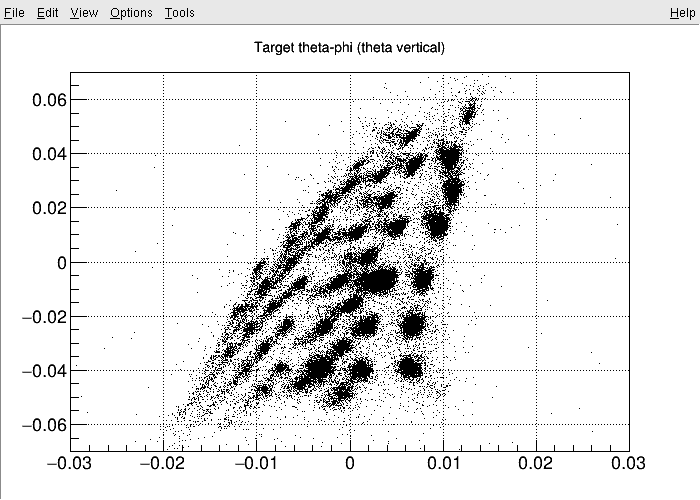
\includegraphics[width=0.32\linewidth]{minus10_septum_minus10_Q1_right}
    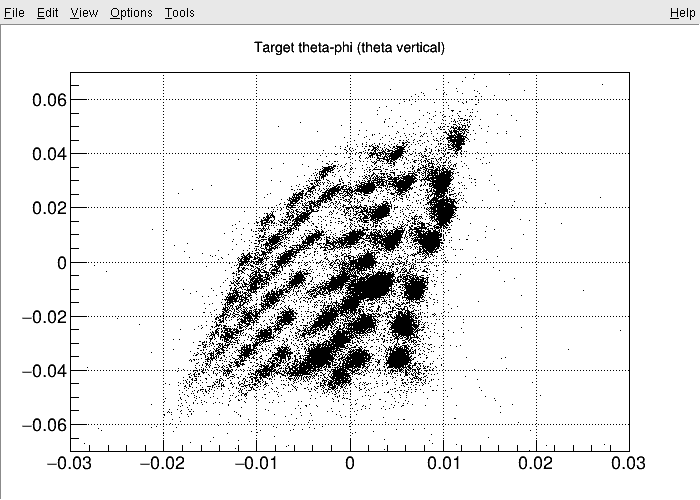
\includegraphics[width=0.32\linewidth]{minus10_septum_nominal_Q1_right}
    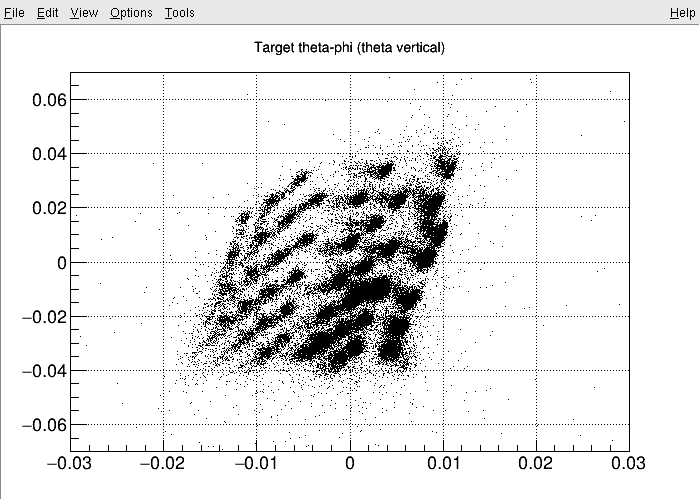
\includegraphics[width=0.32\linewidth]{minus10_septum_plus10_Q1_right}
    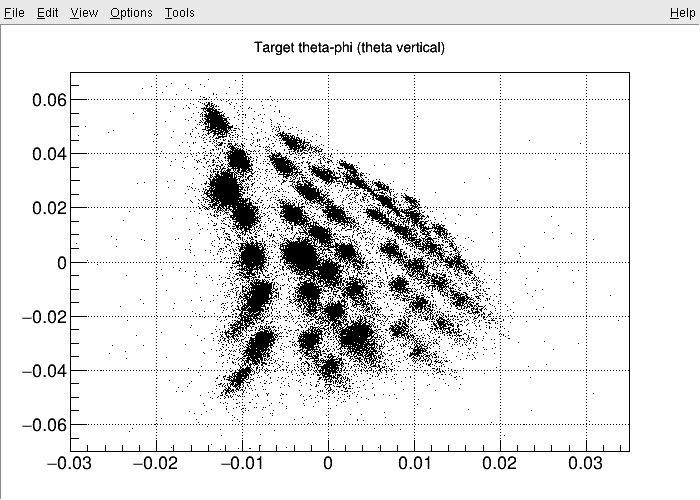
\includegraphics[width=0.32\linewidth]{minus10_septum_minus10_Q1_left}
    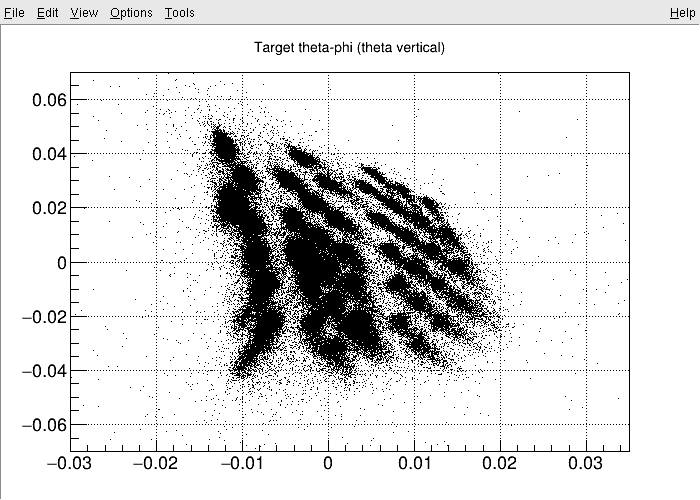
\includegraphics[width=0.32\linewidth]{minus10_septum_nominal_Q1_left}
    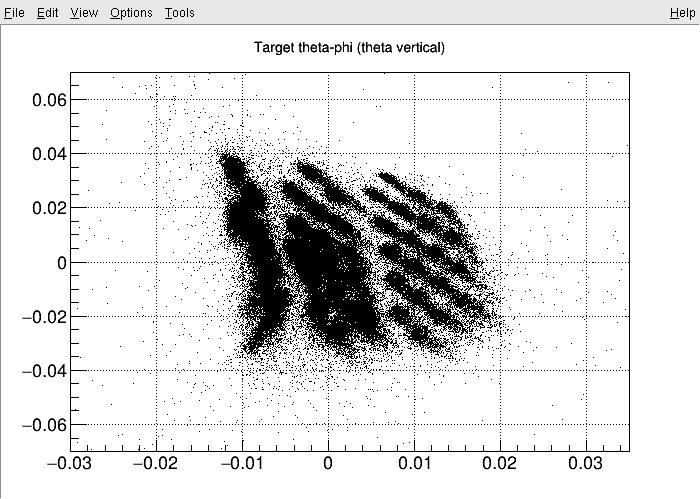
\includegraphics[width=0.32\linewidth]{minus10_septum_plus10_Q1_left}
    \caption{Sieve pattern plots for -10\% septum current
    and varied Q1 current, from left to right: -10\%, nominal and +10\% Q1 current.
    With different Q1 current, the sieve pattern twist, and the central hole 
    shifts in $\theta$, so the septum current is not a good value.}
    \label{fig:central_ray_0}
\end{figure}

\begin{figure}[H]
    \centering
    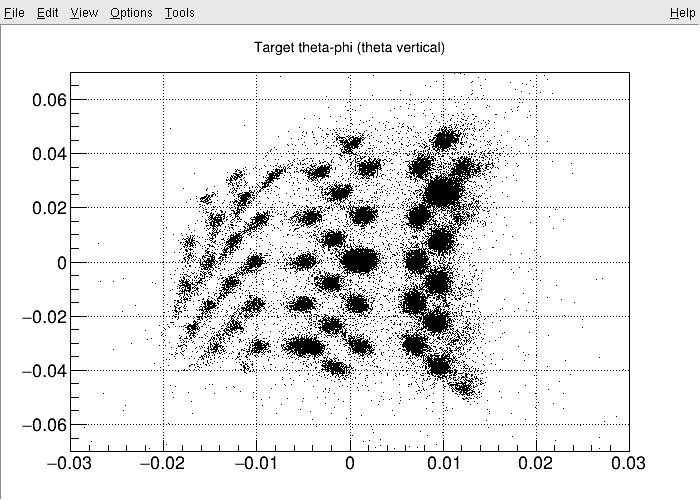
\includegraphics[width=0.32\linewidth]{nominal_septum_minus10_Q1_right}
    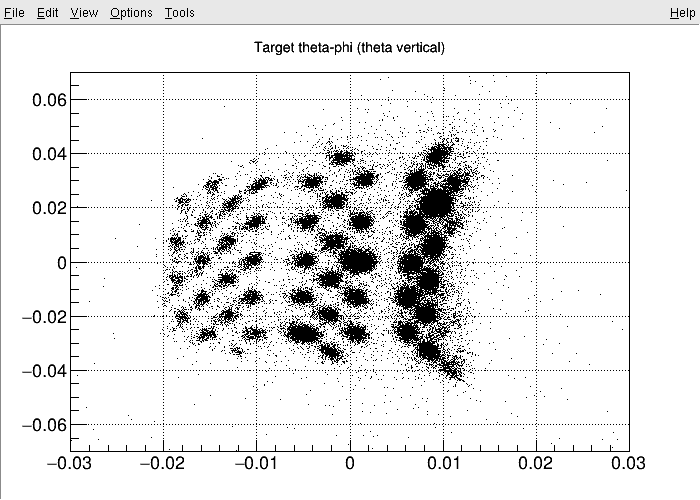
\includegraphics[width=0.32\linewidth]{nominal_septum_nominal_Q1_right}
    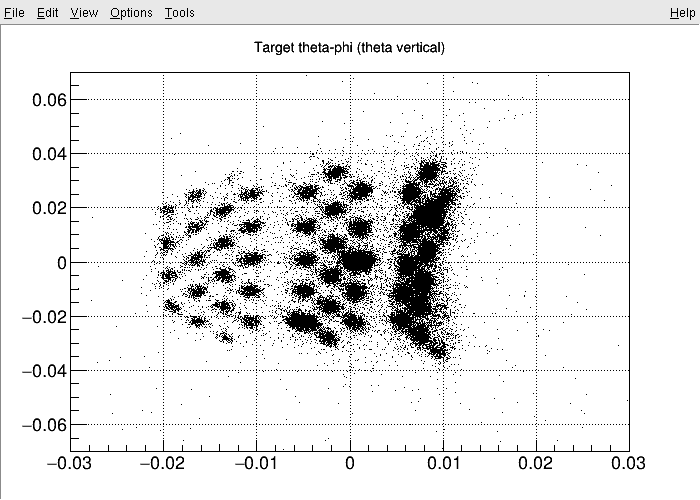
\includegraphics[width=0.32\linewidth]{nominal_septum_plus10_Q1_right}
    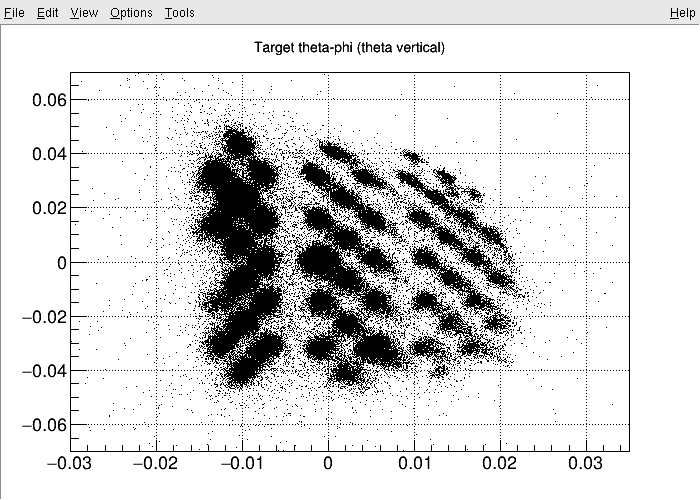
\includegraphics[width=0.32\linewidth]{nominal_septum_minus10_Q1_left}
    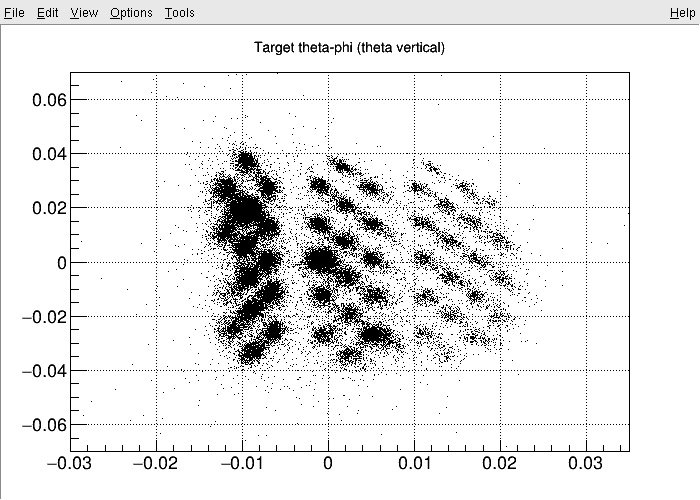
\includegraphics[width=0.32\linewidth]{nominal_septum_nominal_Q1_left}
    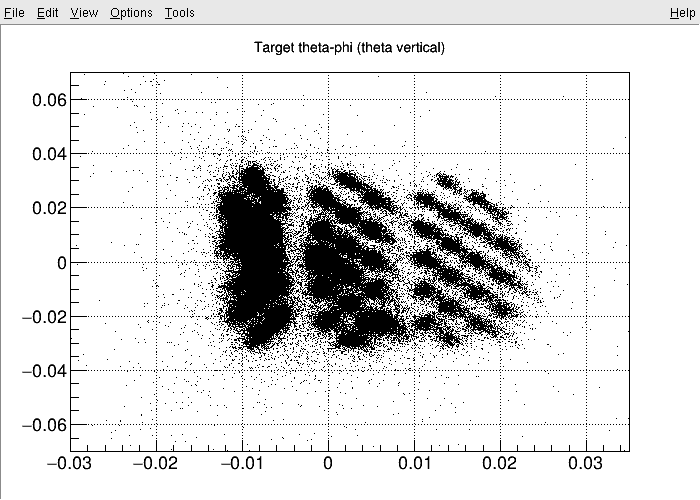
\includegraphics[width=0.32\linewidth]{nominal_septum_plus10_Q1_left}
    \caption{Sieve pattern plots for nominal (scaled from PREX-II setting) septum current
    and varied Q1 current, from left to right: -10\%, nominal and +10\% Q1 current.
    Top row is right arm and bottom row is left arm. With different Q1 current,
    the sieve pattern twist, but the central hole keeps at the same position, 
    which means the central ray goes through the axis of the HRS.}
    \label{fig:central_ray_1}
\end{figure}

Fig. \ref{fig:central_ray_1} told us the nominal septum current and HRS settings was not a bad choice,
so we could move on to inner edge search with this septum nominal value: to
see more inner holes -- holes with largest (smallest) phi in Left (right) arm.
It turned out a 5\% increment from the nominal value gave us the largest 
acceptance, which corresponds to a septum current of: $1.05 \times (333*2.183522/0.95285) = 801.25 \ A$.
\begin{figure}[H]
% https://logbooks.jlab.org/entry/3748464
    \begin{tikzpicture}
	\begin{scope}
	    \node[anchor=south west, inner sep=0] (image) at (0, 0)
	    {	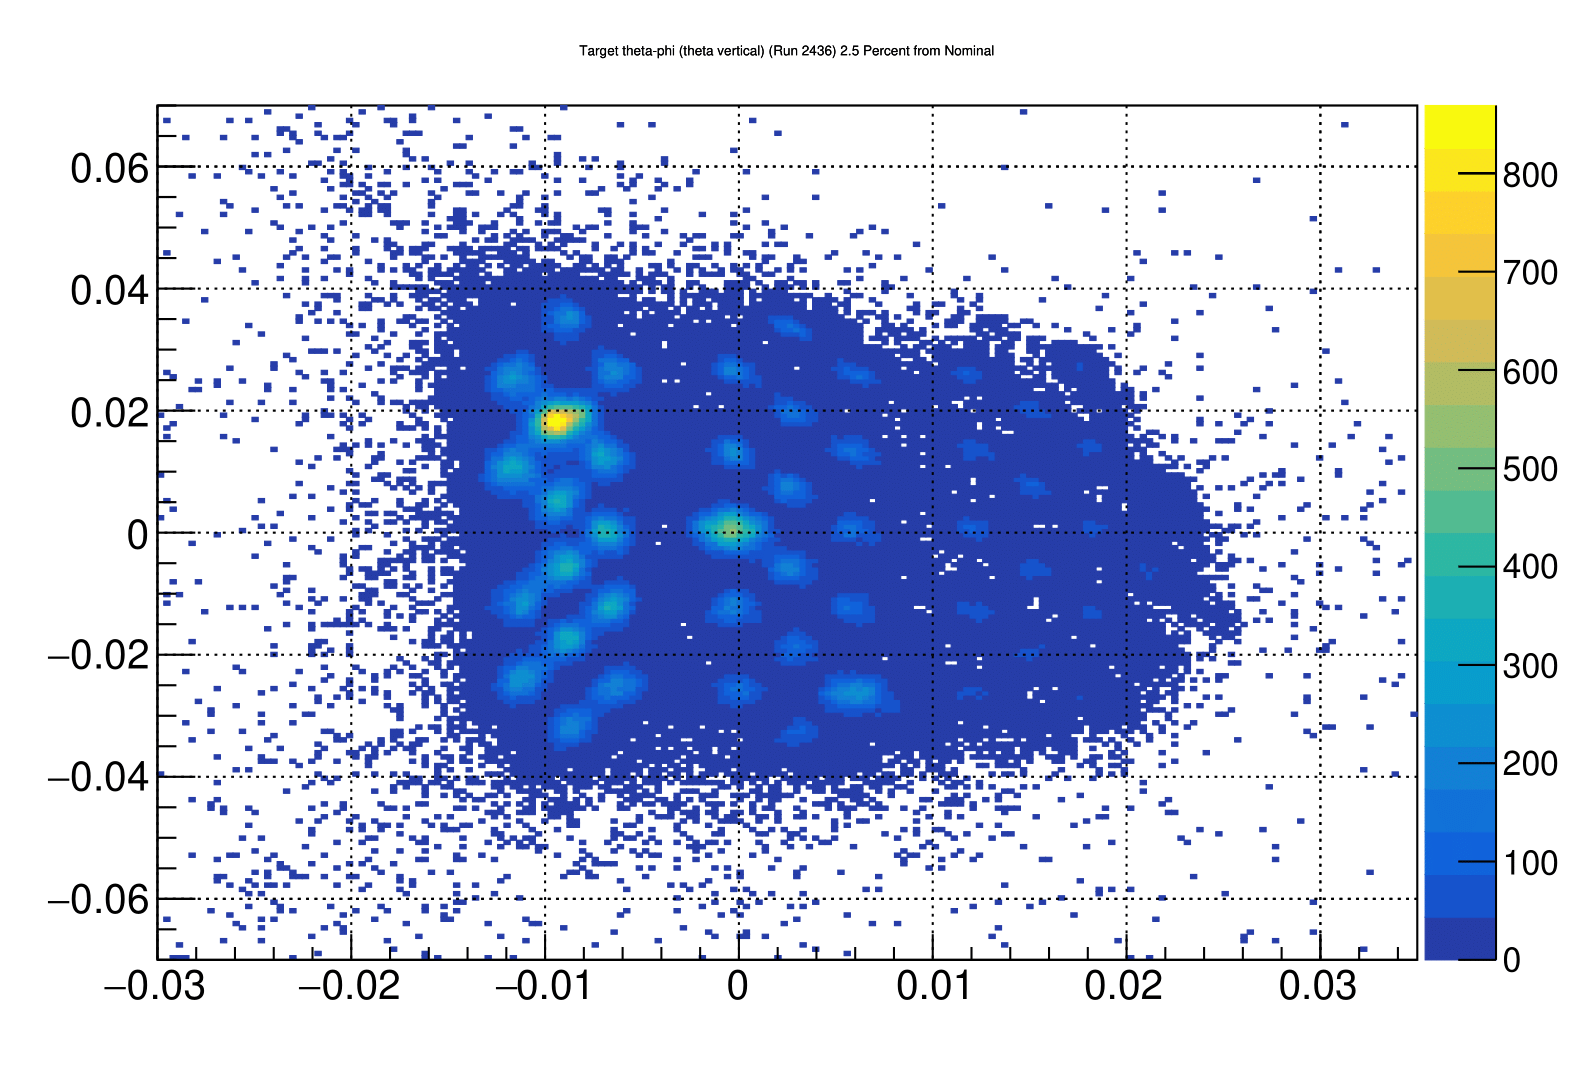
\includegraphics[width=0.49\linewidth]{plus2.5_septum} 
		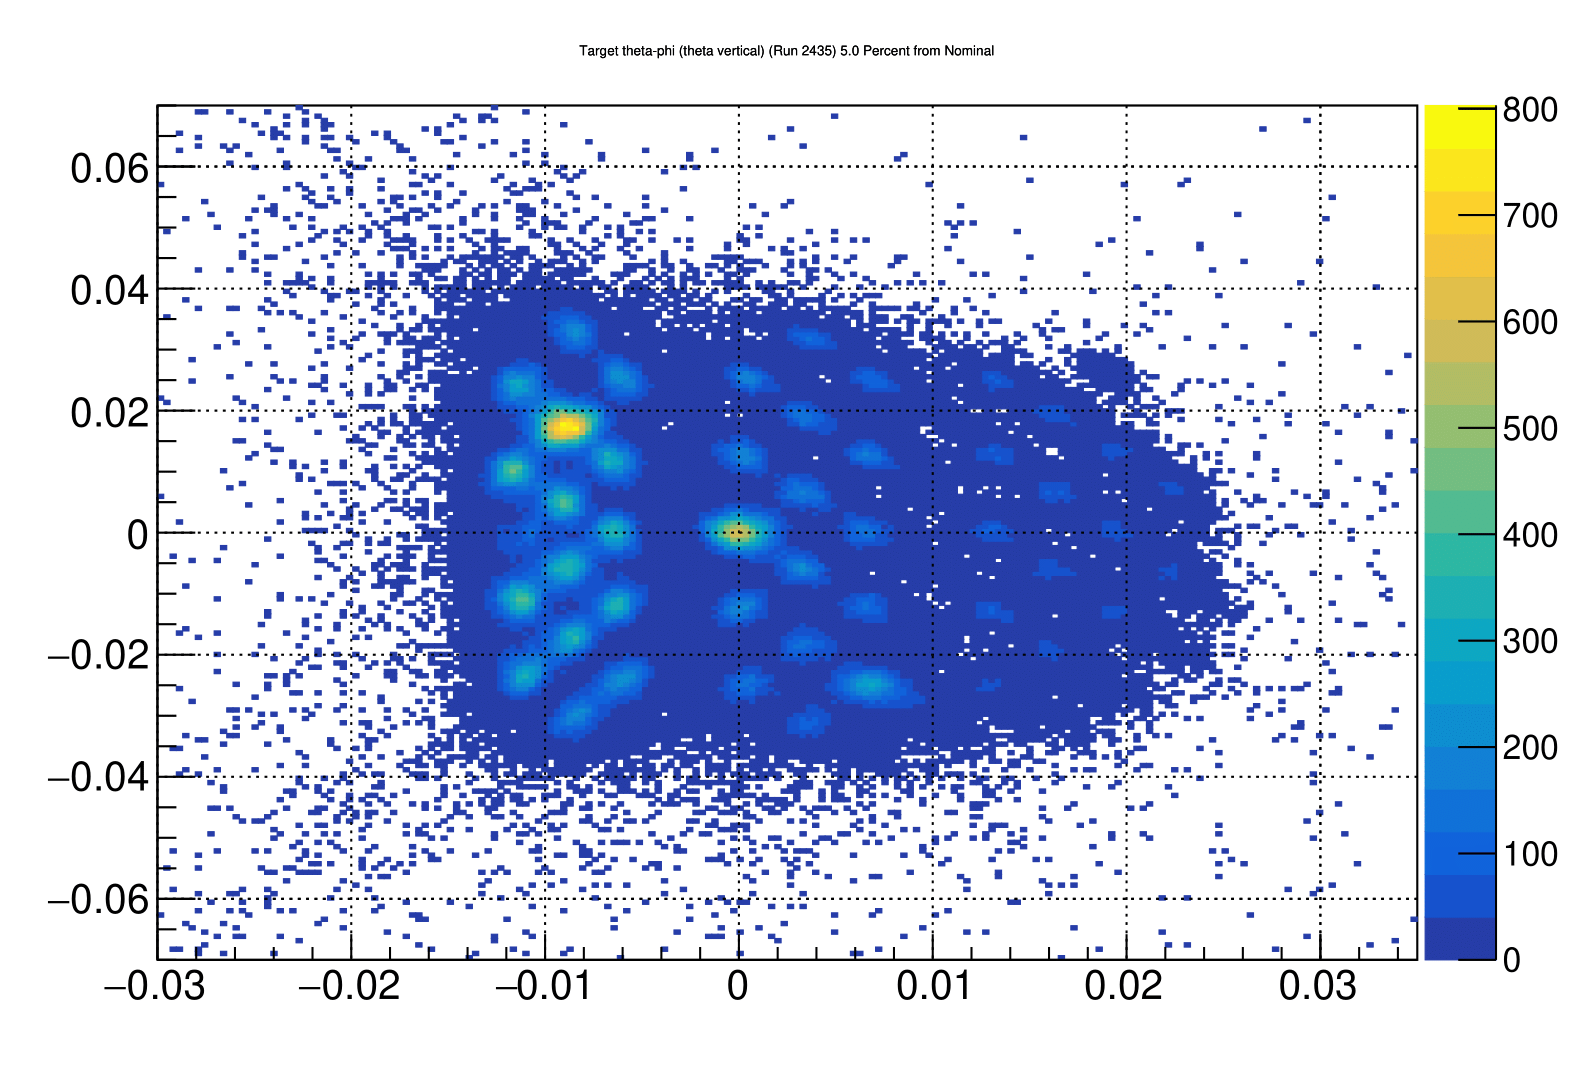
\includegraphics[width=0.49\linewidth]{plus5_septum} 
	    };
	    \begin{scope}[x={(image.south east)}, y={(image.north west)}]
		\draw [thick, Red] (0.67, 0.5) circle (4 pt);
		\draw [thick, Yellow] (0.874, 0.46) circle (4 pt);
		\draw [thick, Yellow] (0.874, 0.55) circle (4 pt);
	    \end{scope}
	\end{scope}
    \end{tikzpicture}
    \begin{tikzpicture}
	\begin{scope}
	    \node[anchor=south west, inner sep=0] (image) at (0, 0)
	    {	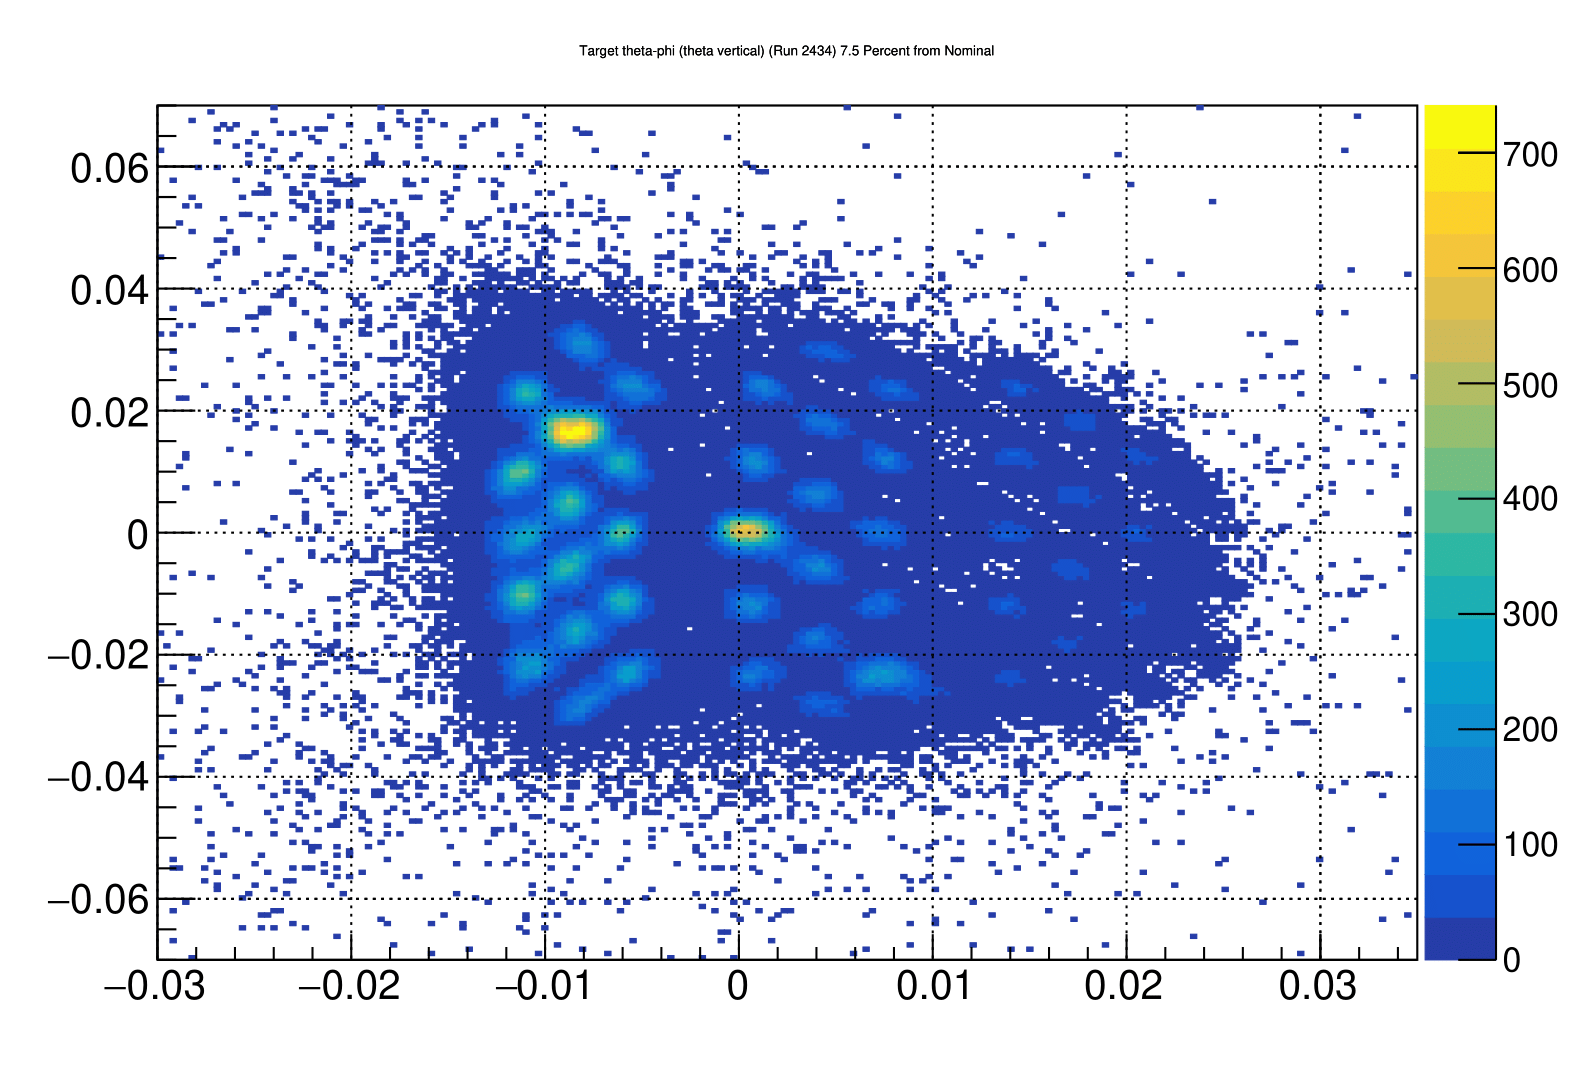
\includegraphics[width=0.49\linewidth]{plus7.5_septum} 
		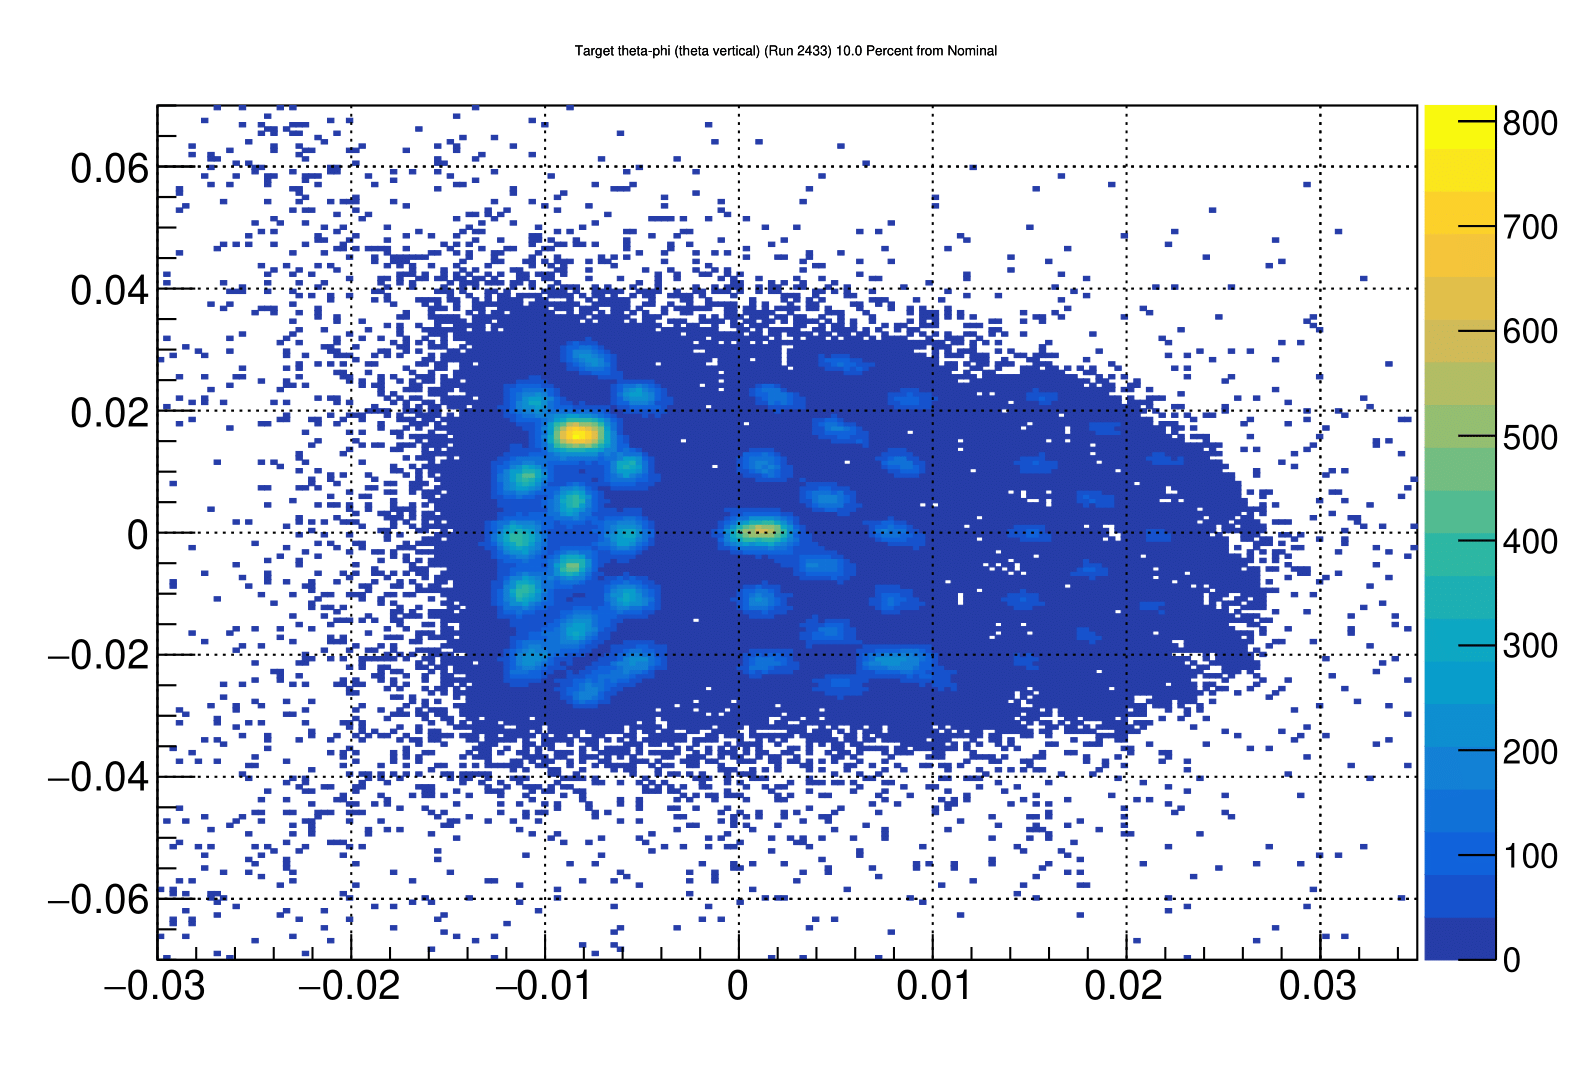
\includegraphics[width=0.49\linewidth]{plus10_septum} 
	    };
	\end{scope}
    \end{tikzpicture}
    \caption{Inner edge search on the left arm. Septum current from top left
    to bottom right: +2.5\%, +5\%, +7.5\%, +10\%. The inner middle hole starts
    to appear since +5\%, and outer holes disappear since 7.5\%, so the best
    septum current was chosen to be +5\%}
\end{figure}

With selected septum current, we continued to minimize beam spot size on the detector
plane, a fine tune of Q1 and Q3 gave us the smallest detector spot size with
Q1 -17\% (-15\%) from the nominal value on left (right) arm, and Q3 -5\% from
the nominal value on both arms, which led to the final CREX tune as shown in
Table~\ref{tab:pcrex_tune}.
\begin{table}[h!]
    \begin{tabular}{c c | c c c | c c c}
	\hline
	& & \multicolumn{3}{c}{Left} & \multicolumn{3}{c}{Right}  \\
	\hline
	Q1(\%)  & Q3 (\%)    & run   & $\sigma_y\ (cm)$  & $\sigma_x\ (cm)$   & run   & $\sigma_y\ (cm)$    & $\sigma_x\ (cm)$    \\
	\hline
	0   & 0	    & 2524  & 0.9604	& 1.634	    & 21604	& 0.009564  & 0.01503 \\
	-5  & 0	    & 2525  & 0.955	& 1.188	    & \multicolumn{3}{c}{Left arm only}    \\
	-10 & 0	    & 2526  & 1.005	& 0.9063    & \multicolumn{3}{c}{Left arm only}    \\ 
	-15 & 0	    & 2527  & 0.1078	& 0.7314    & \multicolumn{3}{c}{Left arm only}    \\ 
	-20 & 0	    & 2528  & 1.182	& 0.6801    & \multicolumn{3}{c}{Left arm only}    \\ 
	\hline                              
	-11 & 0	    & 2529  & 1.012	& 0.8767    & 21609	& 0.009315  & 0.007337	\\
	-12 & 0	    & 2530  & 1.012	& 0.8349    & 21610	& 0.009429  & 0.006957  \\
	-13 & 0	    & 2531  & 1.033	& 0.7835    & 21611	& 0.009526  & 0.006682  \\
	-14 & 0	    & 2532  & 1.057	& 0.7515    & 21612	& 0.009623  & 0.06367   \\
	\hline                              
	-13 & +10   & 2533  & 1.754	& 1.929	    & 21613	& 0.0162    & 0.0215    \\
	-13 & +5    & 2534  & 1.374	& 0.7282    & 21614	& 0.01276   & 0.01174   \\
	-13 & -5    & 2535  & 0.8357	& 0.9751    & 21615	& 0.008422  & 0.008514  \\
	-13 & -10   & 2536  & 0.8855	& 1.482	    & 21616	& 0.008891  & 0.01387   \\
	\hline
	% -13 & -15   & 2537  & 1.133	& 2.042	    & 21617	& 1.141   & 2.051   \\
	-13 & -2    & 2538  & 0.9415	& 0.8761    & 21618	& 0.9117    & 0.7078  \\
	-13 & -4    & 2539  & 0.8602	& 0.9181    & 21619	& 0.8493    & 0.7912  \\
	-13 & -7    & 2540  & 0.8182	& 1.154	    & 21620	& 0.8304    & 1.027   \\
	-13 & -9    & 2541  & 0.8445	& 1.389	    & 21621	& 0.8545    & 1.268   \\
	-15 & -5    & 2542  & 0.8354	& 0.8869    & 21622	& 0.827	    & 0.7563  \\
	\hline
	-15 (R);-17 (L)	& -5	&2543	& 0.8409	& 0.8315  & 21623 & 0.8382	& 0.7615  \\
	\hline
    \end{tabular}
    \caption{Beam spot size with different HRS settings.}
\end{table}

%%%%%%%%%%%%%%%%%%%%%%%%%%%%%%%%%%%%%%%%%%%%%%%%
\subsection{Simulation}
The simulation was not exactly the reproduction of reality. We used GEANT4 to
simulate the geometry of each component based on the designed values, the
septum magnetic field was scaled from a field map file sampled from the septum
at $j_0 = -1320\ A/cm^2$: % FIXME why?
% https://prex.jlab.org/DocDB/0001/000160/001/g4hrs_tune.pdf
\begin{equation}
    B'_{xyz} = \frac{J}{J_0} \times \frac{P}{P_0} \times B_{xyz}
\end{equation}
The same for HRS field: % how to know HRS field at each position
\begin{equation}
    B'_{i = Q1, Q2, D, Q3} = \frac{P}{P_0} \times B_i
\end{equation}

Using this construction, we could firstly vary the septum current to choose the
one that most matched the data, then scanned through collimator shift and pinch point
shift to select the best model.

\begin{figure}[H]
    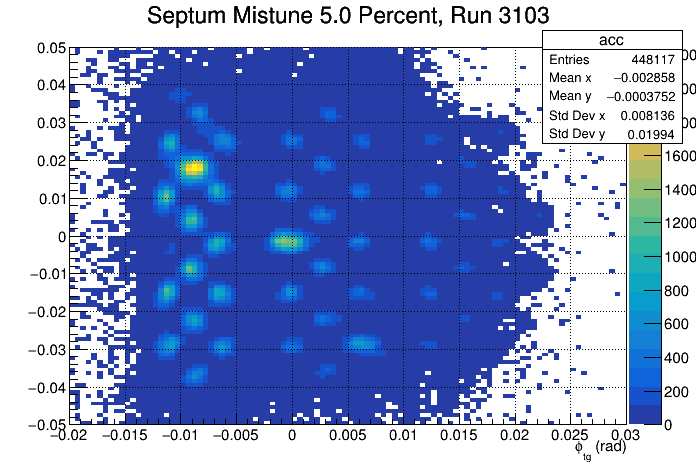
\includegraphics[width=0.49\linewidth]{sieve_run3103}
    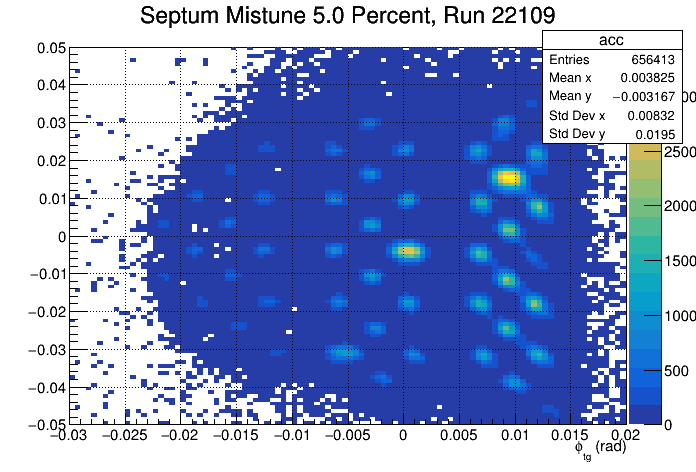
\includegraphics[width=0.49\linewidth]{sieve_run22109}
    \caption{Sieve plot of CREX tune. Centered at (-0.3, -1.5), the new beam 
    position for the new target.}
\end{figure}

Somewhat expected, a coarse scan through the septum told us the septum range
for best model: around 0-5\% above the nominal value.
\begin{figure}[H]
    \begin{tikzpicture}
	\begin{scope}
	    \node[anchor=south west, inner sep=0] (image) at (0, 0)
	    {	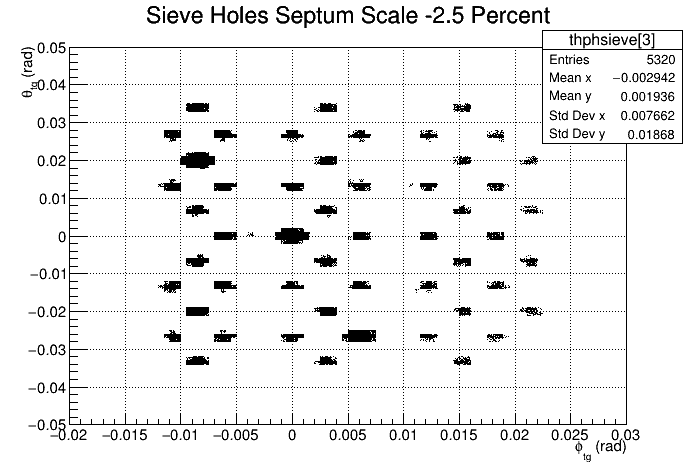
\includegraphics[width=0.49\linewidth]{sieve_sim_minus2.5_left} 
		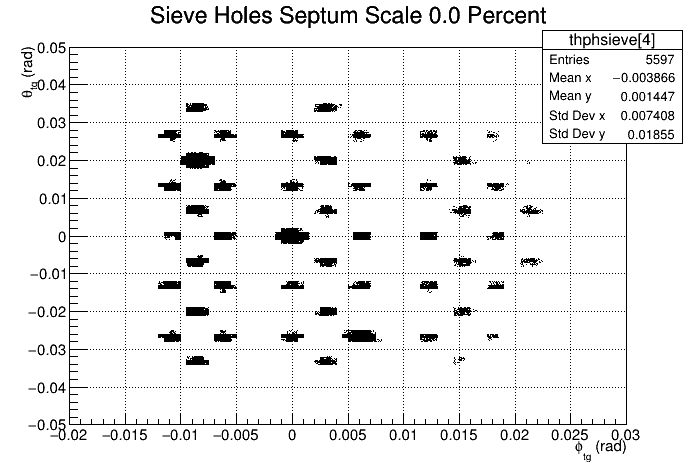
\includegraphics[width=0.49\linewidth]{sieve_sim_nominal_left} 
	    };
	\end{scope}
	\begin{scope}[x={(image.south east)}, y={(image.north west)}]
	    \draw [thick, Red] (0.12, 0.5) circle (4 pt);
	    \draw [thick, Red] (0.33, 0.78) circle (4 pt);
	    \draw [thick, Red] (0.33, 0.23) circle (4 pt);
	    \draw [thick, Red] (0.353, 0.715) circle (4 pt);
	    \draw [thick, Red] (0.353, 0.28) circle (4 pt);
	    \draw [thick, Red] (0.378, 0.655) circle (4 pt);
	    \draw [thick, Red] (0.378, 0.336) circle (4 pt);

	    \draw [thick, Red] (0.83, 0.232) circle (4 pt);
	    \draw [thick, Red] (0.855, 0.715) circle (4 pt);
	    \draw [thick, Red] (0.855, 0.282) circle (4 pt);
	\end{scope}
    \end{tikzpicture}
    \begin{tikzpicture}
	\begin{scope}
	    \node[anchor=south west, inner sep=0] (image) at (0, 0)
	    {	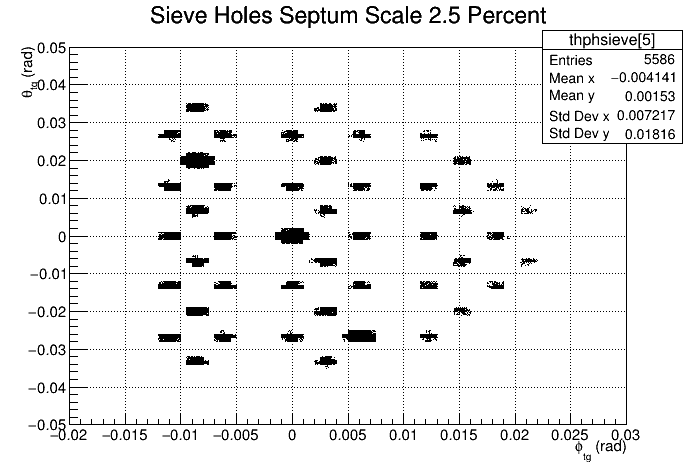
\includegraphics[width=0.49\linewidth]{sieve_sim_plus2.5_left} 
		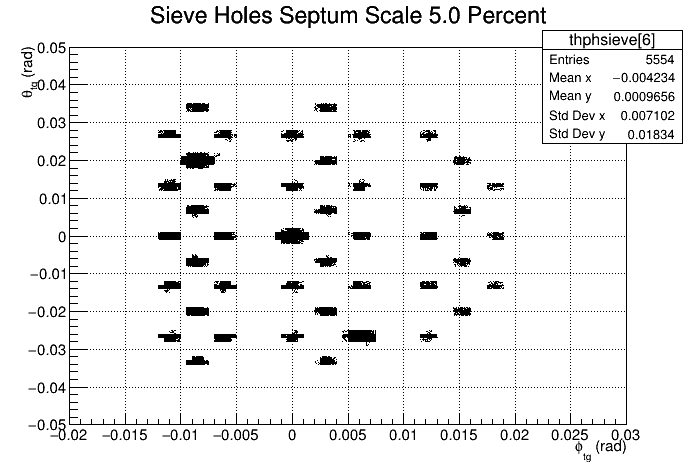
\includegraphics[width=0.49\linewidth]{sieve_sim_plus5_left} 
	    };
	\end{scope}
	\begin{scope}[x={(image.south east)}, y={(image.north west)}]
	    \draw [thick, Red] (0.88, 0.45) circle (4 pt);
	    \draw [thick, Red] (0.88, 0.55) circle (4 pt);
	\end{scope}
    \end{tikzpicture}
    \caption{Sieve pattern plots from simulation with different septum current.}
\end{figure}

\begin{figure}[H]
    \centering
    \begin{tikzpicture}
	\begin{scope}
	    \node[anchor=south west, inner sep=0] (image) at (0, 0)
	    {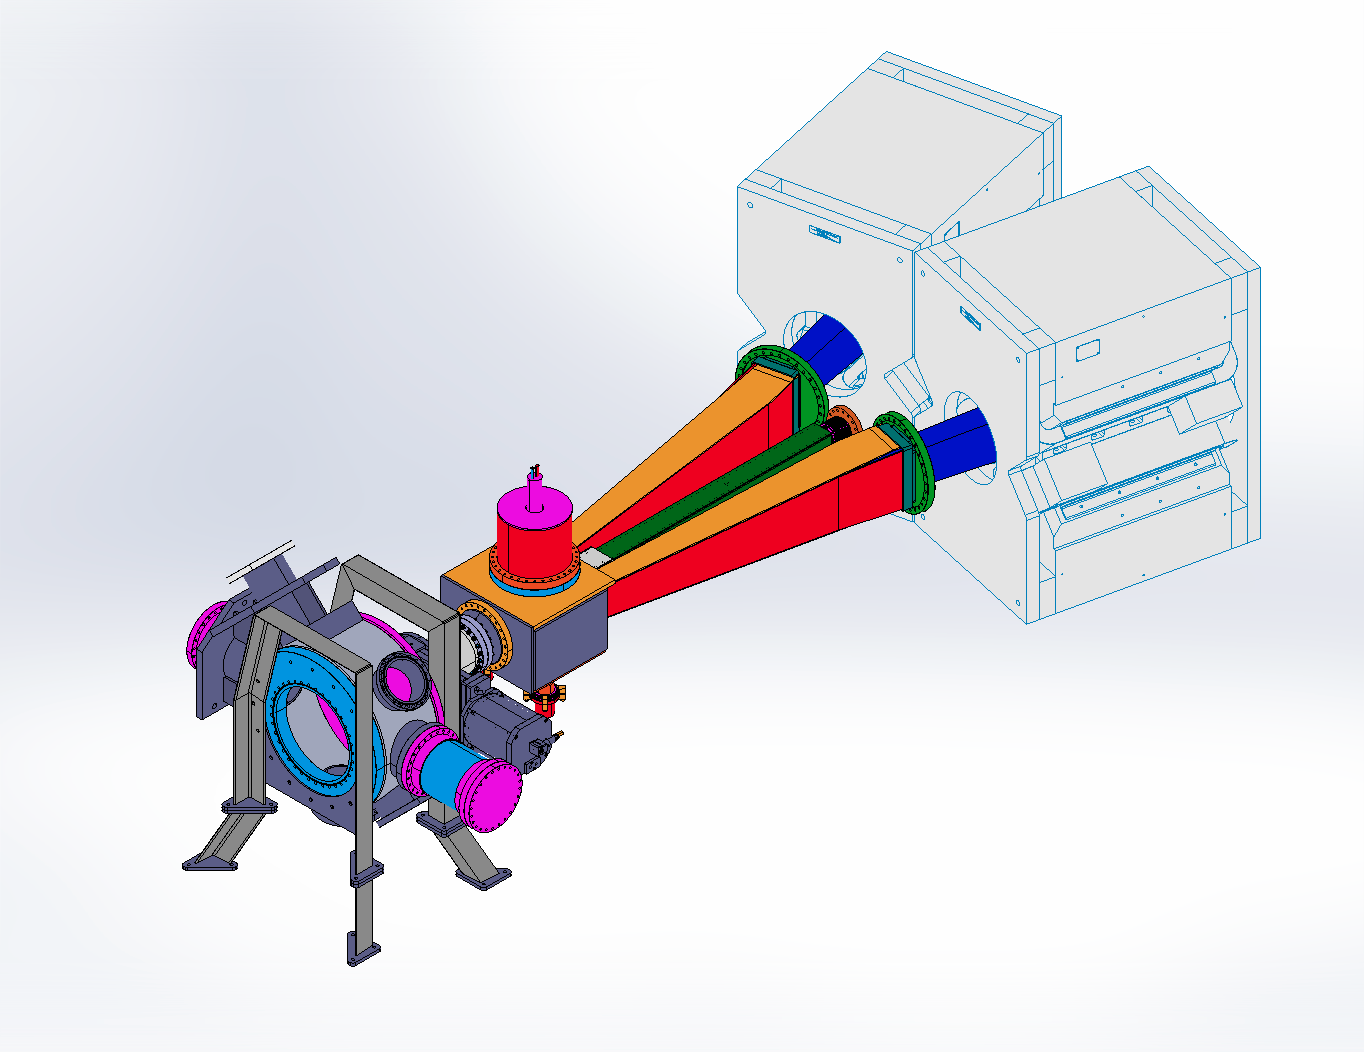
\includegraphics[width=0.5\linewidth]{pivot_region_0}};
	    \begin{scope}[x={(image.south east)},y={(image.north west)}]
		\draw[red,ultra thick] (0.44,0.44) circle (0.17 cm);
		\draw [-latex, thick, red] (0.46, 0.1) node {\scriptsize{Pinch Point}} -- (0.44,0.39);
		\node[green] (coll) at (0.7, 0.2) {\scriptsize{Collimator}};
		\draw [-latex, thick, green] (coll.north) -- (0.67,0.51);
	    \end{scope}
	\end{scope}
    \end{tikzpicture}
    \caption{Position of the pinch point and the Q1 collimator.}
\end{figure}
Then we can scan through the pinch point and collimator shift with a fine tune
of the septum current (from -1\% to +5\%). The pinch point is the connection point
between the septum beampipe and the collimator box, whose misalignment will affect
the acceptance; another parameter we can tune is the collimator (TCS) y position,
which of course has a large impact on the acceptance. For each simulation, we
will compare the average scattering angle $\theta_{lab}$, $Q^2$ and asymmetry to
that of optics data.

\begin{figure}[H]
    \centering
    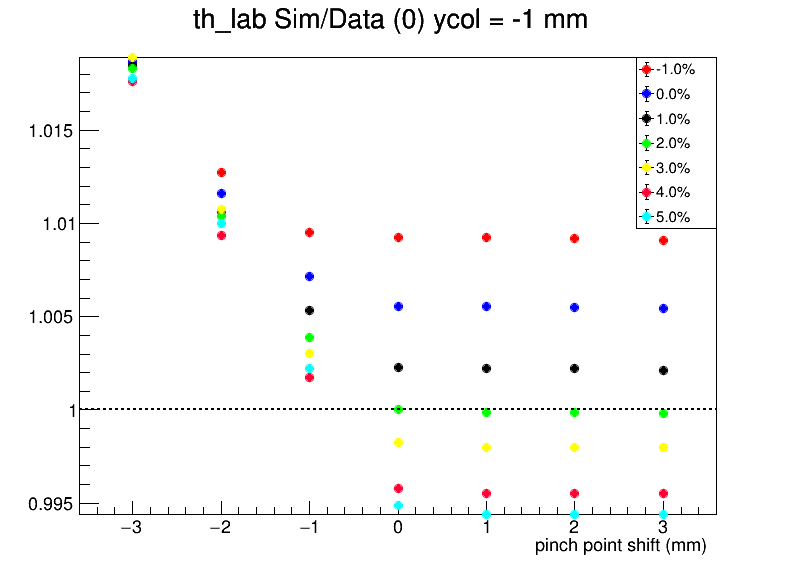
\includegraphics[width=0.32\linewidth]{pinch_scan_th_lab_-1_run0}
    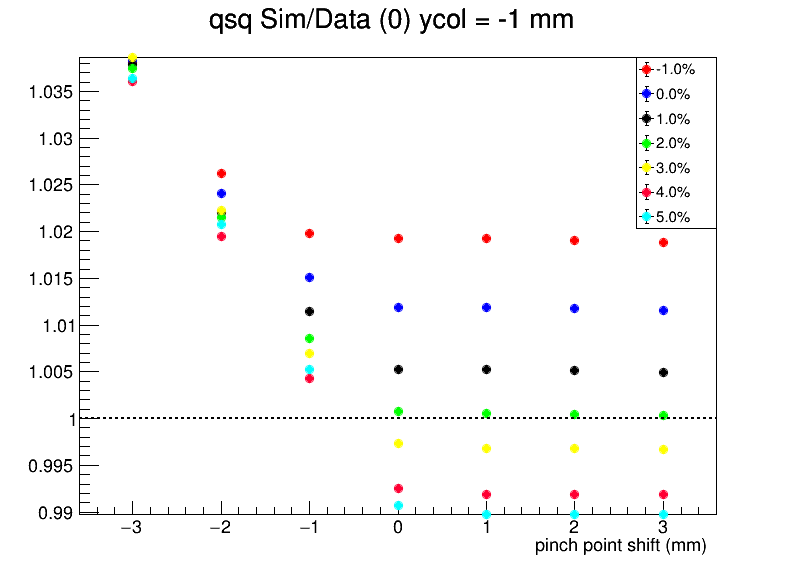
\includegraphics[width=0.32\linewidth]{pinch_scan_qsq_-1_run0}
    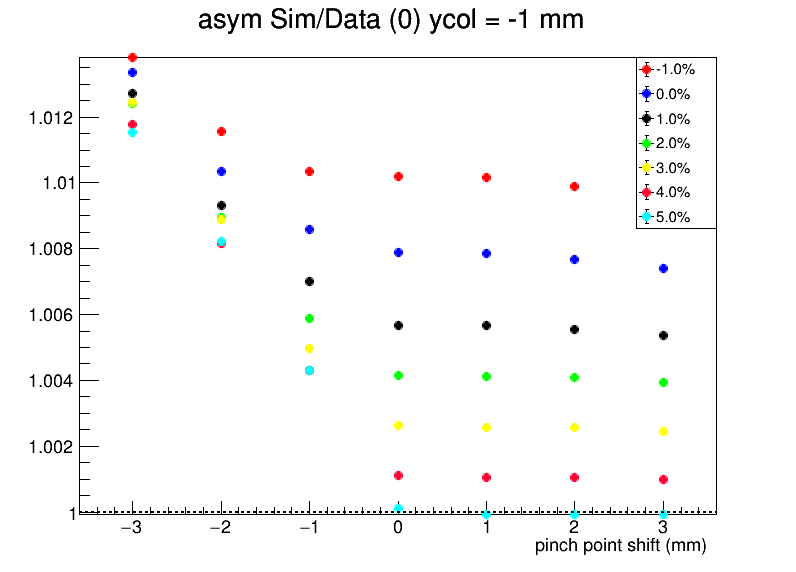
\includegraphics[width=0.32\linewidth]{pinch_scan_asym_-1_run0}
    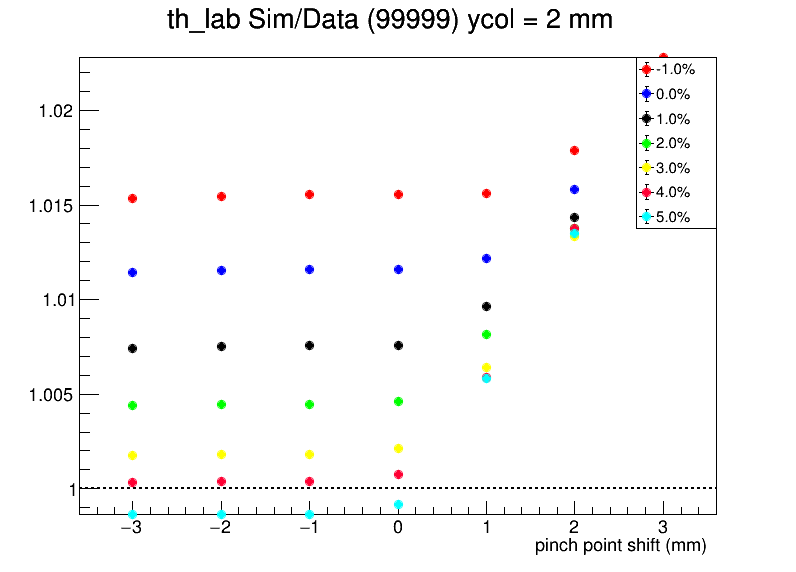
\includegraphics[width=0.32\linewidth]{pinch_scan_th_lab_2_run99999}
    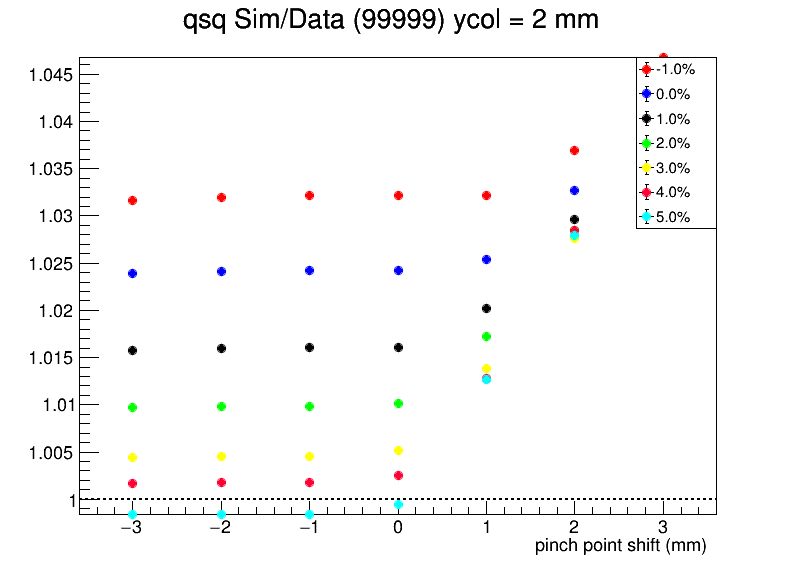
\includegraphics[width=0.32\linewidth]{pinch_scan_qsq_2_run99999}
    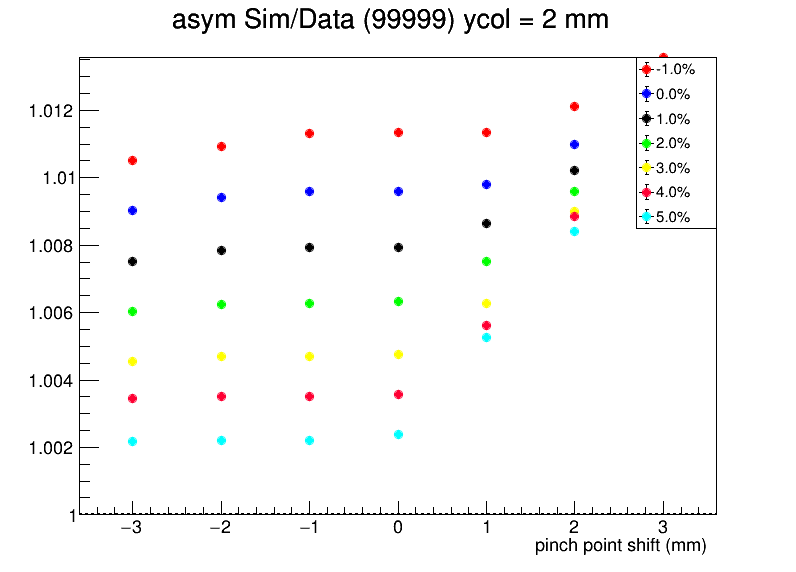
\includegraphics[width=0.32\linewidth]{pinch_scan_asym_2_run99999}
    \caption{Ratio of simulation to data average value for 
    $\theta_{lab}$, $Q^2$ and $\CA$. Top (bottom) row for left (right) arm.
    % FIXME: average over which runs?
    }
    \label{fig:pinch_scan}
\end{figure}

As shown in Fig. \ref{fig:pinch_scan}, when we shift the pinch point toward the
beam pipe (from negative values to positive values for left arm, opposite for 
right arm), the acceptance increases until the nominal value, and then saturates. 
Similar trend was seen for shift of Q1 collimator.
\begin{figure}[H]
    \centering
    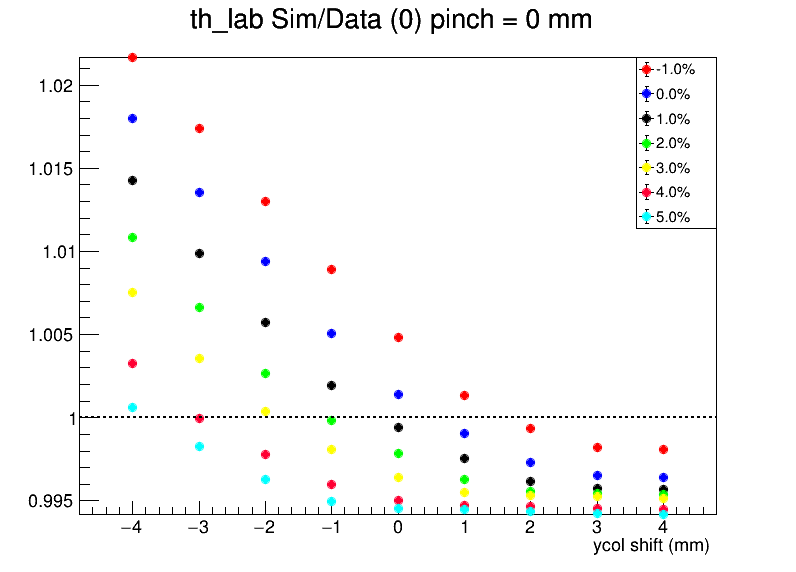
\includegraphics[width=0.49\linewidth]{col_scan_th_lab_0_run0}
    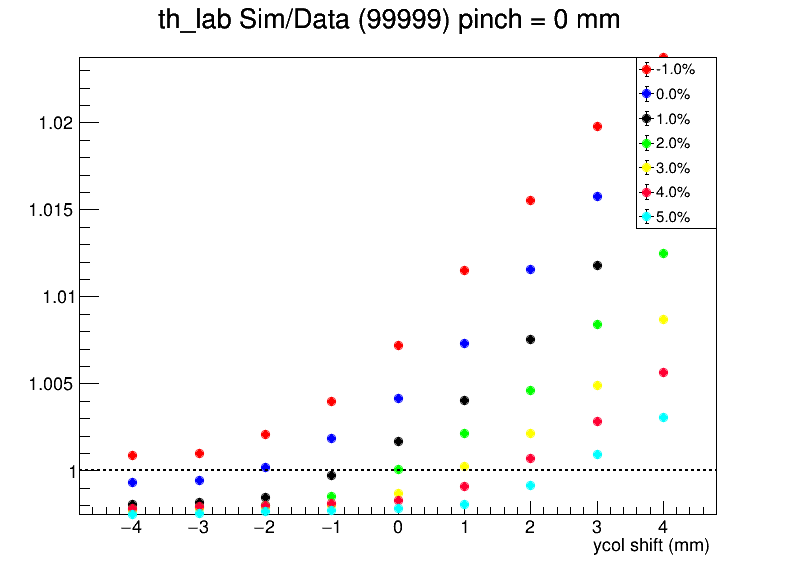
\includegraphics[width=0.49\linewidth]{col_scan_th_lab_0_run99999}
\end{figure}

Various correction was applied to the simulation values. That includes the position
difference between the production target and the calibration target, which was
$20\ mm$ downstream the production \Ca target; and the correction caused by
the database, which was optimized on one beam position ($x_0, y_0$):
\begin{equation}
    \phi_a = \phi_r + 0.5\ mrad/mm \times (x - x_0) + 0.5\ mrad/mm \times (y - y_0)
\end{equation}
(x, y) is the actual beam position. $\phi_a$ and $\phi_r$ are actual and reconstructed
$\phi_{tg}$. An extra acceptance was added to the right arm to get a better 
match.

From the ratio plot, we selected the best model which had the smallest difference
between simulation and data in $\theta_{lab}$ and $Q^2$:
\begin{table}[h!]
    \centering
    \begin{tabular}{c | c c c c}
	\hline
	    & septum & col shift ($mm$)	& pinch point shift ($mm$)	\\
	\hline
	LHRS	& +2\%	& -1	& 0 \\
	RHRS	& +5\%	& 2	& 0 \\
	\hline
    \end{tabular}
\end{table}

We can check the $\theta_{lab}$ for the best models
\begin{figure}[H]
    \centering
    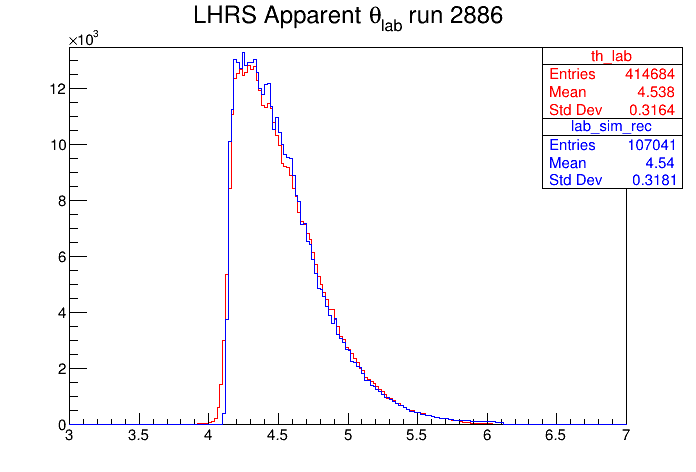
\includegraphics[width=0.49\linewidth]{best_model_run2886_th_lab}
    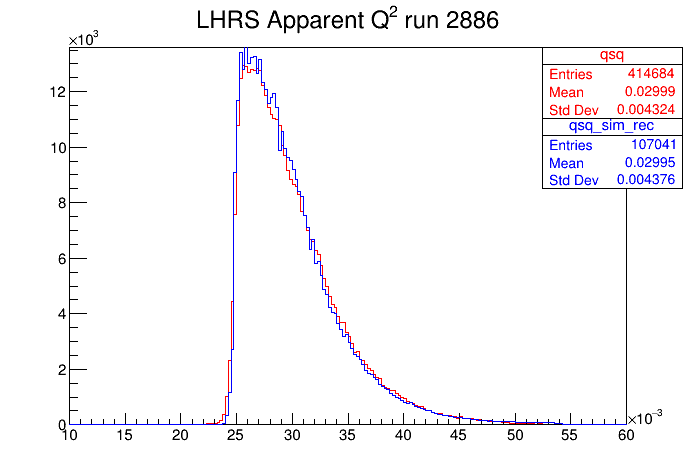
\includegraphics[width=0.49\linewidth]{best_model_run2886_qsq}
    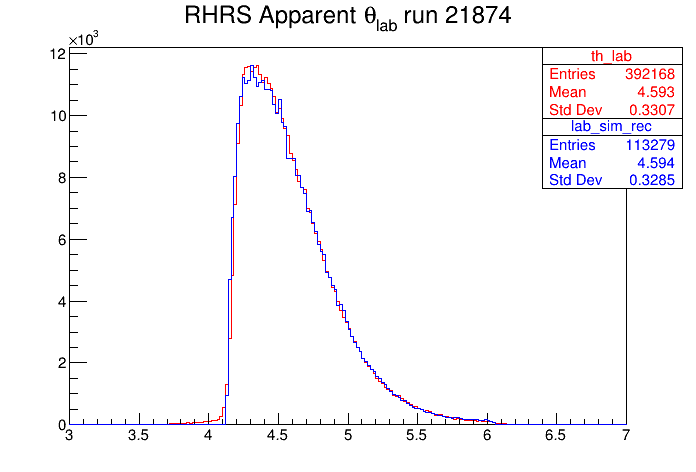
\includegraphics[width=0.49\linewidth]{best_model_run21874_th_lab}
    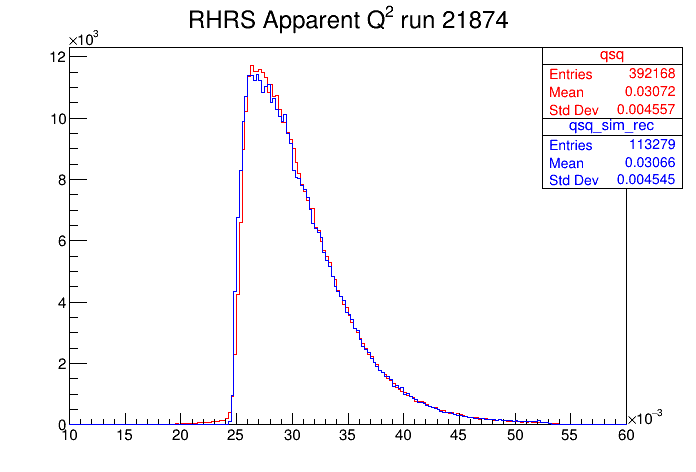
\includegraphics[width=0.49\linewidth]{best_model_run21874_qsq}
    \caption{$\theta_{lab}$ and $Q^2$ comparison between best models and data (apparent values).}
\end{figure}
% We can also check the difference between the vertex values and data:
% \begin{figure}
%     \centering
%     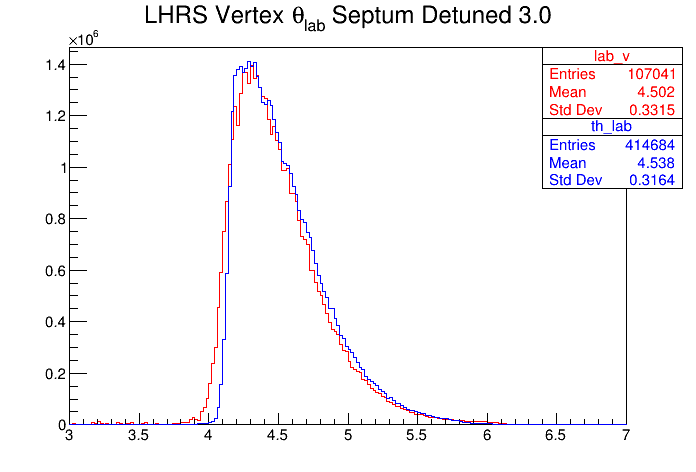
\includegraphics[width=0.49\linewidth]{p3_-2_0_0.0_run2886_th_lab_v}
%     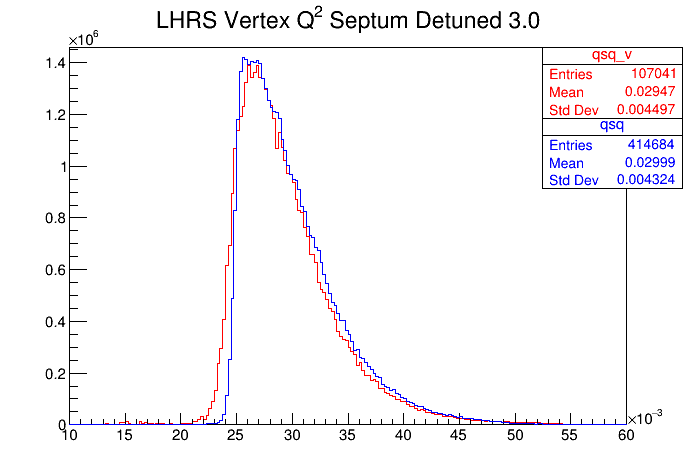
\includegraphics[width=0.49\linewidth]{p3_-2_0_0.0_run2886_qsq_v}
%     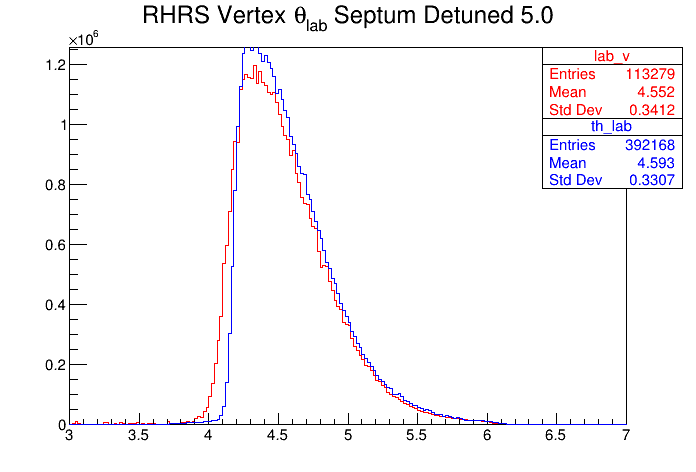
\includegraphics[width=0.49\linewidth]{p5_0_-1_0.0_run21874_th_lab_v}
%     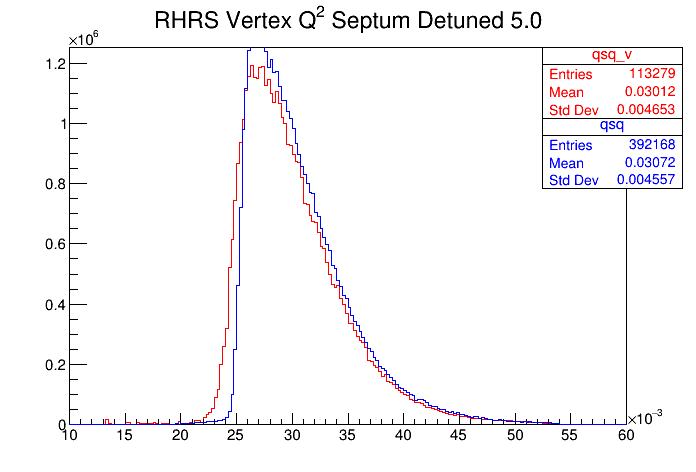
\includegraphics[width=0.49\linewidth]{p5_0_-1_0.0_run21874_qsq_v}
%     \caption{$\theta_{lab}$ and $Q^2$ comparison between best models and data (apparent values).}
% \end{figure}

Using this best models, we can calculate the acceptance function as Eq.~\ref{eq:acceptance_definition}:
\begin{figure}[H]
    \centering
    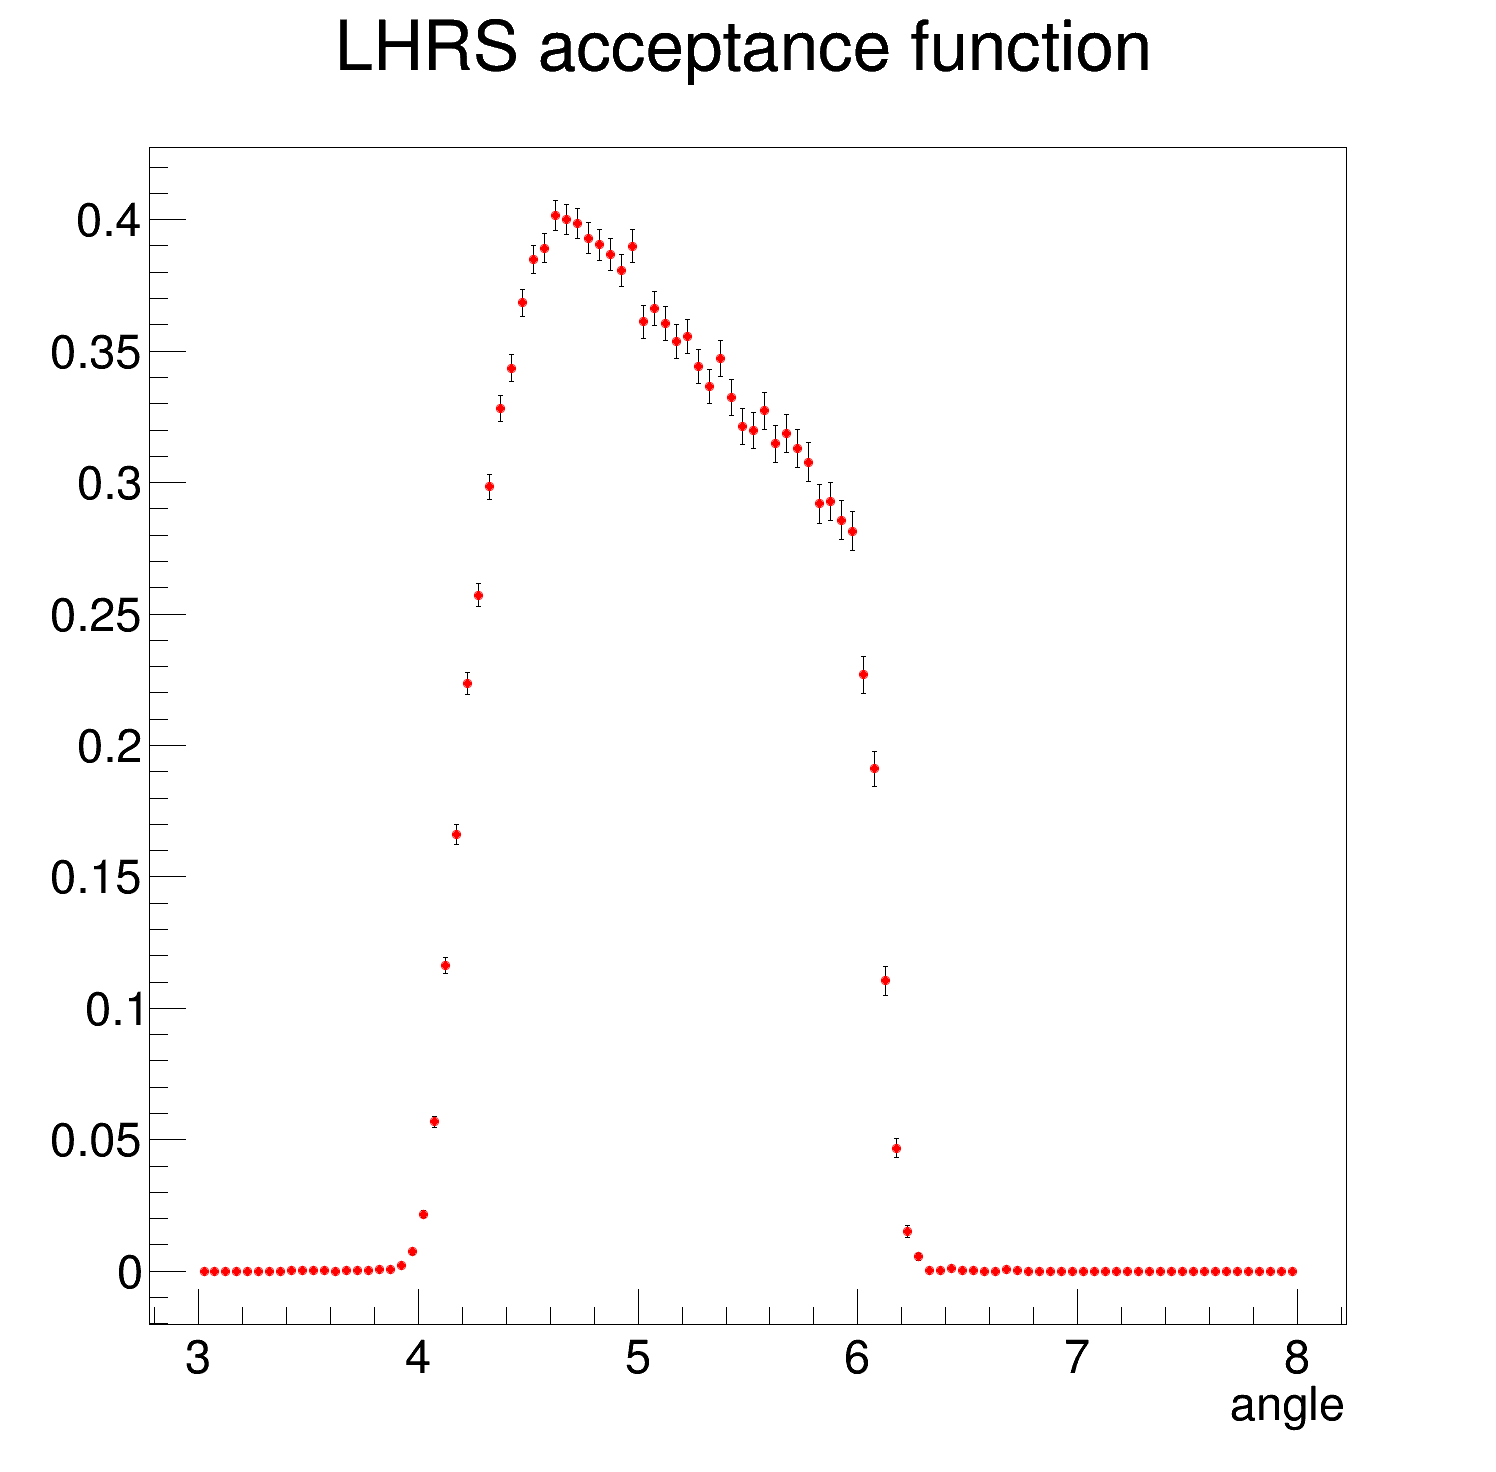
\includegraphics[width=0.49\linewidth]{acc1_L_p2_-1_0_0.0}
    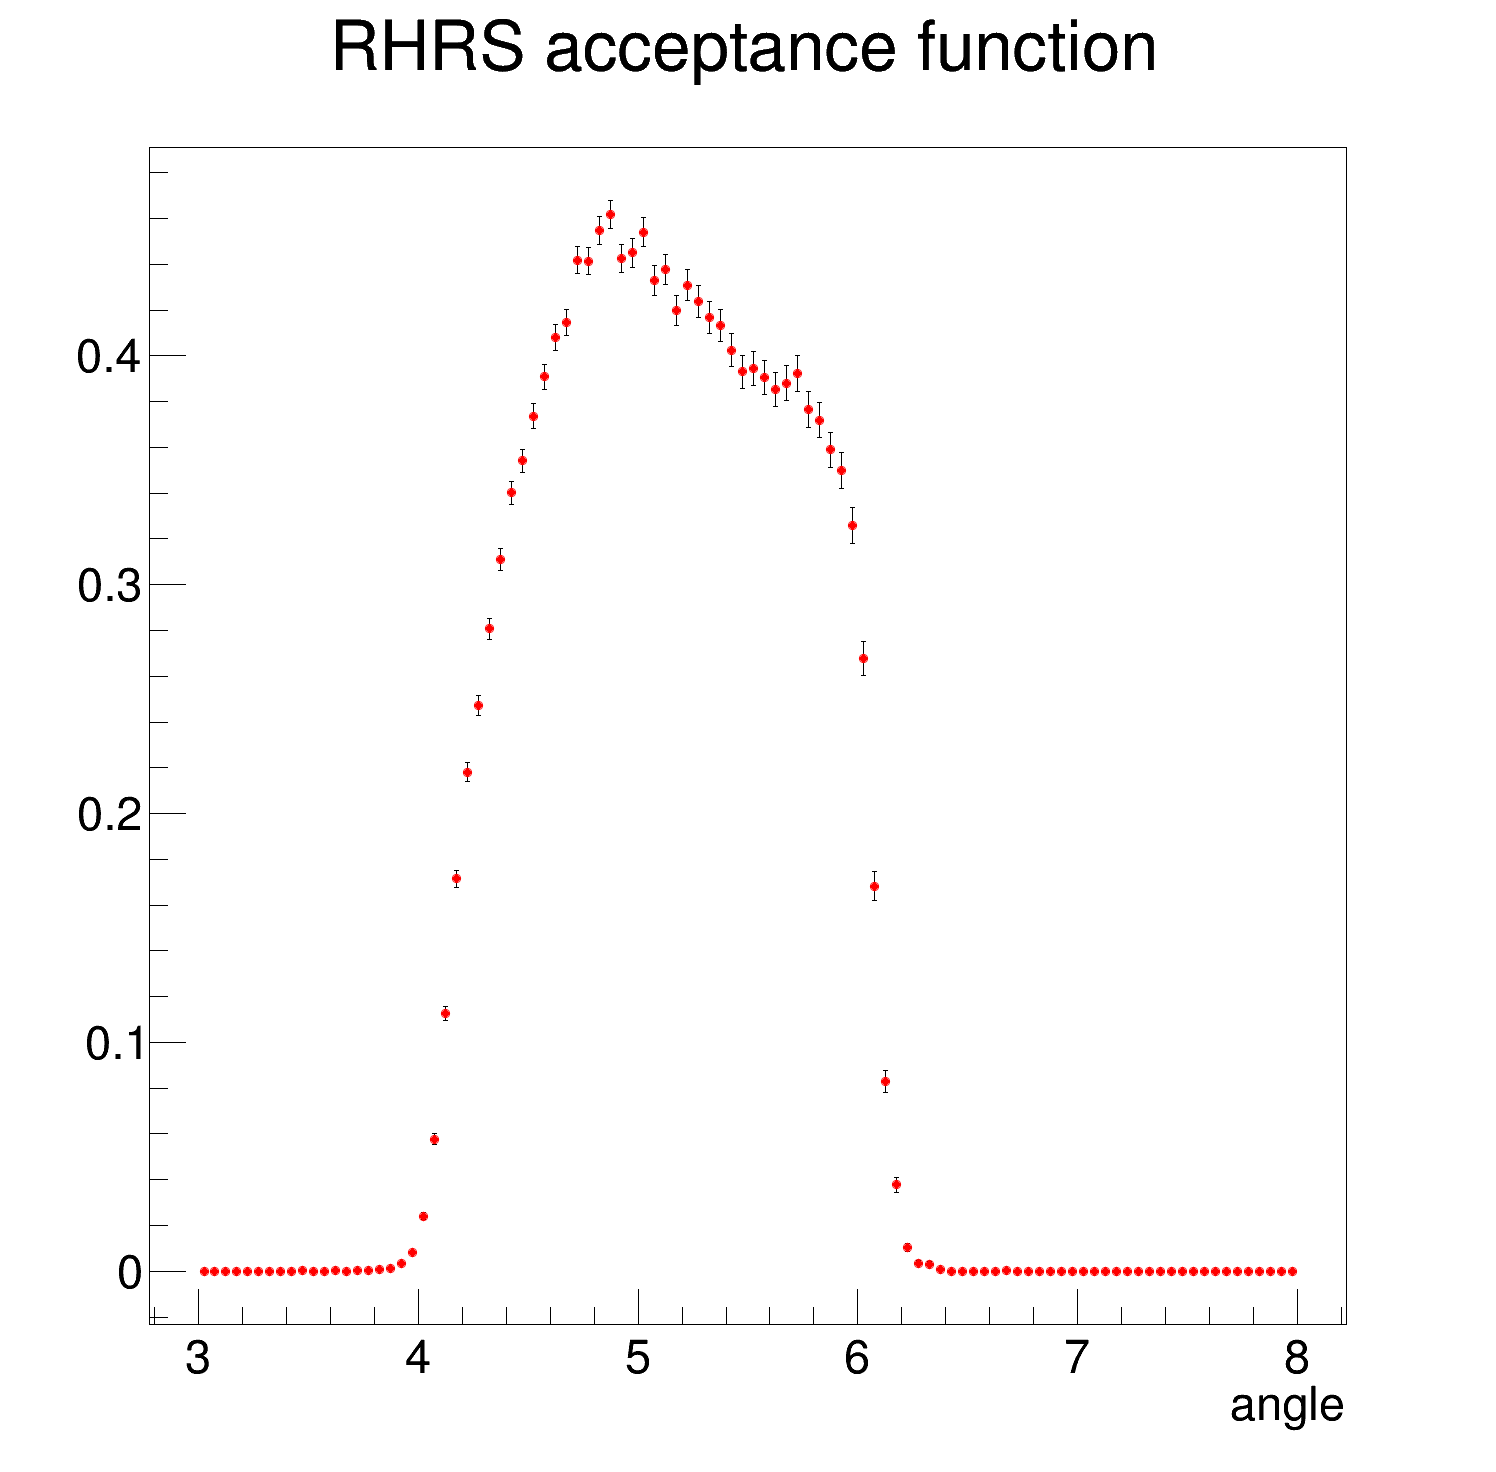
\includegraphics[width=0.49\linewidth]{acc1_R_p5_2_0_0.0}
    \caption{Acceptance function extracted using the best models.}
\end{figure}

%%%%%%%%%%%%%%%%%%%%%%%%
\subsubsection{Non-Linearity}
\begin{equation}
    Y = I + \alpha I^2 + \beta I^3 + \gamma I^4 + \cdots
\end{equation}
Non-linearity: $\alpha$, reduce it 
\begin{itemize}
    \item $\alpha=0.0028$ for Compton $\gamma$ detector
    % https://prex.jlab.org/DocDB/0002/000273/002/Cornejo_and_Quinn_ComptonPhoton_CREX_PREX_Nov_2018.pdf
\end{itemize}
% \subsection{tg variables}
